\documentclass[twoside]{book}

% Packages required by doxygen
\usepackage{calc}
\usepackage{doxygen}
\usepackage{graphicx}
\usepackage[utf8]{inputenc}
\usepackage{makeidx}
\usepackage{multicol}
\usepackage{multirow}
\usepackage{textcomp}
\usepackage[table]{xcolor}

% Font selection
\usepackage[T1]{fontenc}
\usepackage{mathptmx}
\usepackage[scaled=.90]{helvet}
\usepackage{courier}
\usepackage{amssymb}
\usepackage{sectsty}
\renewcommand{\familydefault}{\sfdefault}
\allsectionsfont{%
  \fontseries{bc}\selectfont%
  \color{darkgray}%
}
\renewcommand{\DoxyLabelFont}{%
  \fontseries{bc}\selectfont%
  \color{darkgray}%
}

% Page & text layout
\usepackage{geometry}
\geometry{%
  a4paper,%
  top=2.5cm,%
  bottom=2.5cm,%
  left=2.5cm,%
  right=2.5cm%
}
\tolerance=750
\hfuzz=15pt
\hbadness=750
\setlength{\emergencystretch}{15pt}
\setlength{\parindent}{0cm}
\setlength{\parskip}{0.2cm}
\makeatletter
\renewcommand{\paragraph}{%
  \@startsection{paragraph}{4}{0ex}{-1.0ex}{1.0ex}{%
    \normalfont\normalsize\bfseries\SS@parafont%
  }%
}
\renewcommand{\subparagraph}{%
  \@startsection{subparagraph}{5}{0ex}{-1.0ex}{1.0ex}{%
    \normalfont\normalsize\bfseries\SS@subparafont%
  }%
}
\makeatother

% Headers & footers
\usepackage{fancyhdr}
\pagestyle{fancyplain}
\fancyhead[LE]{\fancyplain{}{\bfseries\thepage}}
\fancyhead[CE]{\fancyplain{}{}}
\fancyhead[RE]{\fancyplain{}{\bfseries\leftmark}}
\fancyhead[LO]{\fancyplain{}{\bfseries\rightmark}}
\fancyhead[CO]{\fancyplain{}{}}
\fancyhead[RO]{\fancyplain{}{\bfseries\thepage}}
\fancyfoot[LE]{\fancyplain{}{}}
\fancyfoot[CE]{\fancyplain{}{}}
\fancyfoot[RE]{\fancyplain{}{\bfseries\scriptsize Generated on Thu May 8 2014 17\-:03\-:53 for My Project by Doxygen }}
\fancyfoot[LO]{\fancyplain{}{\bfseries\scriptsize Generated on Thu May 8 2014 17\-:03\-:53 for My Project by Doxygen }}
\fancyfoot[CO]{\fancyplain{}{}}
\fancyfoot[RO]{\fancyplain{}{}}
\renewcommand{\footrulewidth}{0.4pt}
\renewcommand{\chaptermark}[1]{%
  \markboth{#1}{}%
}
\renewcommand{\sectionmark}[1]{%
  \markright{\thesection\ #1}%
}

% Indices & bibliography
\usepackage{natbib}
\usepackage[titles]{tocloft}
\setcounter{tocdepth}{3}
\setcounter{secnumdepth}{5}
\makeindex

% Hyperlinks (required, but should be loaded last)
\usepackage{ifpdf}
\ifpdf
  \usepackage[pdftex,pagebackref=true]{hyperref}
\else
  \usepackage[ps2pdf,pagebackref=true]{hyperref}
\fi
\hypersetup{%
  colorlinks=true,%
  linkcolor=blue,%
  citecolor=blue,%
  unicode%
}

% Custom commands
\newcommand{\clearemptydoublepage}{%
  \newpage{\pagestyle{empty}\cleardoublepage}%
}


%===== C O N T E N T S =====

\begin{document}

% Titlepage & ToC
\hypersetup{pageanchor=false}
\pagenumbering{roman}
\begin{titlepage}
\vspace*{7cm}
\begin{center}%
{\Large My Project }\\
\vspace*{1cm}
{\large Generated by Doxygen 1.8.6}\\
\vspace*{0.5cm}
{\small Thu May 8 2014 17:03:53}\\
\end{center}
\end{titlepage}
\clearemptydoublepage
\tableofcontents
\clearemptydoublepage
\pagenumbering{arabic}
\hypersetup{pageanchor=true}

%--- Begin generated contents ---
\chapter{Class Index}
\section{Class List}
Here are the classes, structs, unions and interfaces with brief descriptions\-:\begin{DoxyCompactList}
\item\contentsline{section}{\hyperlink{classCoinSlot}{Coin\-Slot} }{\pageref{classCoinSlot}}{}
\item\contentsline{section}{\hyperlink{structDestination}{Destination} }{\pageref{structDestination}}{}
\item\contentsline{section}{\hyperlink{classDestinationCollection}{Destination\-Collection} }{\pageref{classDestinationCollection}}{}
\item\contentsline{section}{\hyperlink{classPriceComputer}{Price\-Computer} }{\pageref{classPriceComputer}}{}
\item\contentsline{section}{\hyperlink{classRefoundComputer}{Refound\-Computer} }{\pageref{classRefoundComputer}}{}
\item\contentsline{section}{\hyperlink{classTicketMachine}{Ticket\-Machine} }{\pageref{classTicketMachine}}{}
\end{DoxyCompactList}

\chapter{File Index}
\section{File List}
Here is a list of all files with brief descriptions\-:\begin{DoxyCompactList}
\item\contentsline{section}{\hyperlink{calculator_8cpp}{calculator.\-cpp} }{\pageref{calculator_8cpp}}{}
\item\contentsline{section}{\hyperlink{calculator_8h}{calculator.\-h} }{\pageref{calculator_8h}}{}
\item\contentsline{section}{\hyperlink{console__input_8cpp}{console\-\_\-input.\-cpp} }{\pageref{console__input_8cpp}}{}
\item\contentsline{section}{\hyperlink{console__input_8h}{console\-\_\-input.\-h} }{\pageref{console__input_8h}}{}
\item\contentsline{section}{\hyperlink{fraction_8cpp}{fraction.\-cpp} }{\pageref{fraction_8cpp}}{}
\item\contentsline{section}{\hyperlink{fraction_8h}{fraction.\-h} }{\pageref{fraction_8h}}{}
\item\contentsline{section}{\hyperlink{main_8cpp}{main.\-cpp} }{\pageref{main_8cpp}}{}
\item\contentsline{section}{\hyperlink{main_8h}{main.\-h} }{\pageref{main_8h}}{}
\end{DoxyCompactList}

\chapter{Class Documentation}
\hypertarget{structDate}{\section{Date Struct Reference}
\label{structDate}\index{Date@{Date}}
}


{\ttfamily \#include $<$date.\-h$>$}

\subsection*{Public Attributes}
\begin{DoxyCompactItemize}
\item 
int \hyperlink{structDate_a5b192adcabf2b2871e3f0b76c1ec1601}{day}
\item 
int \hyperlink{structDate_a533843e07c6ac8d19fee9b16f5336ba2}{month}
\item 
int \hyperlink{structDate_a3eeced2ed56bc95d56782b9e738db8ea}{year}
\end{DoxyCompactItemize}


\subsection{Member Data Documentation}
\hypertarget{structDate_a5b192adcabf2b2871e3f0b76c1ec1601}{\index{Date@{Date}!day@{day}}
\index{day@{day}!Date@{Date}}
\subsubsection[{day}]{\setlength{\rightskip}{0pt plus 5cm}int Date\-::day}}\label{structDate_a5b192adcabf2b2871e3f0b76c1ec1601}
\hypertarget{structDate_a533843e07c6ac8d19fee9b16f5336ba2}{\index{Date@{Date}!month@{month}}
\index{month@{month}!Date@{Date}}
\subsubsection[{month}]{\setlength{\rightskip}{0pt plus 5cm}int Date\-::month}}\label{structDate_a533843e07c6ac8d19fee9b16f5336ba2}
\hypertarget{structDate_a3eeced2ed56bc95d56782b9e738db8ea}{\index{Date@{Date}!year@{year}}
\index{year@{year}!Date@{Date}}
\subsubsection[{year}]{\setlength{\rightskip}{0pt plus 5cm}int Date\-::year}}\label{structDate_a3eeced2ed56bc95d56782b9e738db8ea}


The documentation for this struct was generated from the following file\-:\begin{DoxyCompactItemize}
\item 
\hyperlink{date_8h}{date.\-h}\end{DoxyCompactItemize}

\chapter{File Documentation}
\hypertarget{_8ycm__extra__conf_8py}{\section{.ycm\-\_\-extra\-\_\-conf.\-py File Reference}
\label{_8ycm__extra__conf_8py}\index{.\-ycm\-\_\-extra\-\_\-conf.\-py@{.\-ycm\-\_\-extra\-\_\-conf.\-py}}
}
\subsection*{Functions}
\begin{DoxyCompactItemize}
\item 
def \hyperlink{_8ycm__extra__conf_8py_a28506547e5aee74e22557e0d523fbba7}{Directory\-Of\-This\-Script}
\item 
def \hyperlink{_8ycm__extra__conf_8py_aa17b17787ee25ee278fe0330e8245fb8}{Make\-Relative\-Paths\-In\-Flags\-Absolute}
\item 
def \hyperlink{_8ycm__extra__conf_8py_a38a706def8307cce6e9348c3379274bd}{Is\-Header\-File}
\item 
def \hyperlink{_8ycm__extra__conf_8py_a1c7294d0bfbd409f9d5d418ed3e91a52}{Get\-Compilation\-Info\-For\-File}
\item 
def \hyperlink{_8ycm__extra__conf_8py_af1c9418abf3c686550f9a8be0dc6b2ef}{Flags\-For\-File}
\end{DoxyCompactItemize}
\subsection*{Variables}
\begin{DoxyCompactItemize}
\item 
list \hyperlink{_8ycm__extra__conf_8py_abd73d8e4551f1a637280b3876d1ae2e3}{flags}
\item 
string \hyperlink{_8ycm__extra__conf_8py_a6a4d7e96c7bc9093b406af626b7936a2}{compilation\-\_\-database\-\_\-folder} = ''
\item 
tuple \hyperlink{_8ycm__extra__conf_8py_a64dbaa3229ec575b68ec333442e10cee}{database} = ycm\-\_\-core.\-Compilation\-Database( \hyperlink{_8ycm__extra__conf_8py_a6a4d7e96c7bc9093b406af626b7936a2}{compilation\-\_\-database\-\_\-folder} )
\item 
list \hyperlink{_8ycm__extra__conf_8py_a47014996e1e517071cd0412a22adb123}{S\-O\-U\-R\-C\-E\-\_\-\-E\-X\-T\-E\-N\-S\-I\-O\-N\-S} = \mbox{[} '.cpp', '.cxx', '.cc', '.c', '.m', '.mm' \mbox{]}
\end{DoxyCompactItemize}


\subsection{Function Documentation}
\hypertarget{_8ycm__extra__conf_8py_a28506547e5aee74e22557e0d523fbba7}{\index{.\-ycm\-\_\-extra\-\_\-conf.\-py@{.\-ycm\-\_\-extra\-\_\-conf.\-py}!Directory\-Of\-This\-Script@{Directory\-Of\-This\-Script}}
\index{Directory\-Of\-This\-Script@{Directory\-Of\-This\-Script}!.ycm_extra_conf.py@{.\-ycm\-\_\-extra\-\_\-conf.\-py}}
\subsubsection[{Directory\-Of\-This\-Script}]{\setlength{\rightskip}{0pt plus 5cm}def Directory\-Of\-This\-Script (
\begin{DoxyParamCaption}
{}
\end{DoxyParamCaption}
)}}\label{_8ycm__extra__conf_8py_a28506547e5aee74e22557e0d523fbba7}
\hypertarget{_8ycm__extra__conf_8py_af1c9418abf3c686550f9a8be0dc6b2ef}{\index{.\-ycm\-\_\-extra\-\_\-conf.\-py@{.\-ycm\-\_\-extra\-\_\-conf.\-py}!Flags\-For\-File@{Flags\-For\-File}}
\index{Flags\-For\-File@{Flags\-For\-File}!.ycm_extra_conf.py@{.\-ycm\-\_\-extra\-\_\-conf.\-py}}
\subsubsection[{Flags\-For\-File}]{\setlength{\rightskip}{0pt plus 5cm}def Flags\-For\-File (
\begin{DoxyParamCaption}
\item[{}]{filename, }
\item[{}]{kwargs}
\end{DoxyParamCaption}
)}}\label{_8ycm__extra__conf_8py_af1c9418abf3c686550f9a8be0dc6b2ef}


Here is the call graph for this function\-:\nopagebreak
\begin{figure}[H]
\begin{center}
\leavevmode
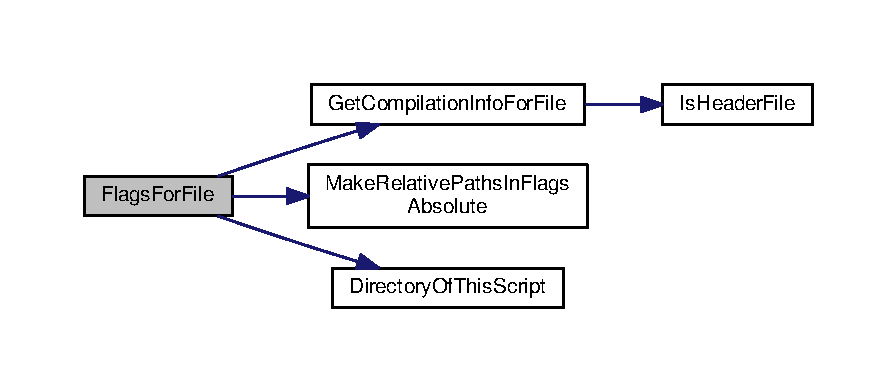
\includegraphics[width=350pt]{_8ycm__extra__conf_8py_af1c9418abf3c686550f9a8be0dc6b2ef_cgraph}
\end{center}
\end{figure}


\hypertarget{_8ycm__extra__conf_8py_a1c7294d0bfbd409f9d5d418ed3e91a52}{\index{.\-ycm\-\_\-extra\-\_\-conf.\-py@{.\-ycm\-\_\-extra\-\_\-conf.\-py}!Get\-Compilation\-Info\-For\-File@{Get\-Compilation\-Info\-For\-File}}
\index{Get\-Compilation\-Info\-For\-File@{Get\-Compilation\-Info\-For\-File}!.ycm_extra_conf.py@{.\-ycm\-\_\-extra\-\_\-conf.\-py}}
\subsubsection[{Get\-Compilation\-Info\-For\-File}]{\setlength{\rightskip}{0pt plus 5cm}def Get\-Compilation\-Info\-For\-File (
\begin{DoxyParamCaption}
\item[{}]{filename}
\end{DoxyParamCaption}
)}}\label{_8ycm__extra__conf_8py_a1c7294d0bfbd409f9d5d418ed3e91a52}


Here is the call graph for this function\-:\nopagebreak
\begin{figure}[H]
\begin{center}
\leavevmode
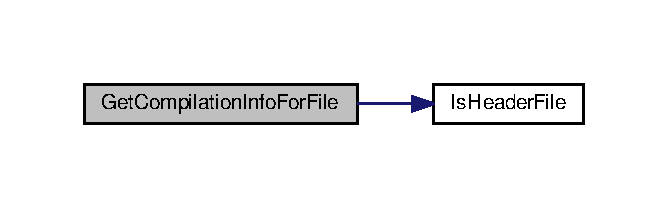
\includegraphics[width=320pt]{_8ycm__extra__conf_8py_a1c7294d0bfbd409f9d5d418ed3e91a52_cgraph}
\end{center}
\end{figure}


\hypertarget{_8ycm__extra__conf_8py_a38a706def8307cce6e9348c3379274bd}{\index{.\-ycm\-\_\-extra\-\_\-conf.\-py@{.\-ycm\-\_\-extra\-\_\-conf.\-py}!Is\-Header\-File@{Is\-Header\-File}}
\index{Is\-Header\-File@{Is\-Header\-File}!.ycm_extra_conf.py@{.\-ycm\-\_\-extra\-\_\-conf.\-py}}
\subsubsection[{Is\-Header\-File}]{\setlength{\rightskip}{0pt plus 5cm}def Is\-Header\-File (
\begin{DoxyParamCaption}
\item[{}]{filename}
\end{DoxyParamCaption}
)}}\label{_8ycm__extra__conf_8py_a38a706def8307cce6e9348c3379274bd}
\hypertarget{_8ycm__extra__conf_8py_aa17b17787ee25ee278fe0330e8245fb8}{\index{.\-ycm\-\_\-extra\-\_\-conf.\-py@{.\-ycm\-\_\-extra\-\_\-conf.\-py}!Make\-Relative\-Paths\-In\-Flags\-Absolute@{Make\-Relative\-Paths\-In\-Flags\-Absolute}}
\index{Make\-Relative\-Paths\-In\-Flags\-Absolute@{Make\-Relative\-Paths\-In\-Flags\-Absolute}!.ycm_extra_conf.py@{.\-ycm\-\_\-extra\-\_\-conf.\-py}}
\subsubsection[{Make\-Relative\-Paths\-In\-Flags\-Absolute}]{\setlength{\rightskip}{0pt plus 5cm}def Make\-Relative\-Paths\-In\-Flags\-Absolute (
\begin{DoxyParamCaption}
\item[{}]{flags, }
\item[{}]{working\-\_\-directory}
\end{DoxyParamCaption}
)}}\label{_8ycm__extra__conf_8py_aa17b17787ee25ee278fe0330e8245fb8}


\subsection{Variable Documentation}
\hypertarget{_8ycm__extra__conf_8py_a6a4d7e96c7bc9093b406af626b7936a2}{\index{.\-ycm\-\_\-extra\-\_\-conf.\-py@{.\-ycm\-\_\-extra\-\_\-conf.\-py}!compilation\-\_\-database\-\_\-folder@{compilation\-\_\-database\-\_\-folder}}
\index{compilation\-\_\-database\-\_\-folder@{compilation\-\_\-database\-\_\-folder}!.ycm_extra_conf.py@{.\-ycm\-\_\-extra\-\_\-conf.\-py}}
\subsubsection[{compilation\-\_\-database\-\_\-folder}]{\setlength{\rightskip}{0pt plus 5cm}string compilation\-\_\-database\-\_\-folder = ''}}\label{_8ycm__extra__conf_8py_a6a4d7e96c7bc9093b406af626b7936a2}
\hypertarget{_8ycm__extra__conf_8py_a64dbaa3229ec575b68ec333442e10cee}{\index{.\-ycm\-\_\-extra\-\_\-conf.\-py@{.\-ycm\-\_\-extra\-\_\-conf.\-py}!database@{database}}
\index{database@{database}!.ycm_extra_conf.py@{.\-ycm\-\_\-extra\-\_\-conf.\-py}}
\subsubsection[{database}]{\setlength{\rightskip}{0pt plus 5cm}database = ycm\-\_\-core.\-Compilation\-Database( {\bf compilation\-\_\-database\-\_\-folder} )}}\label{_8ycm__extra__conf_8py_a64dbaa3229ec575b68ec333442e10cee}
\hypertarget{_8ycm__extra__conf_8py_abd73d8e4551f1a637280b3876d1ae2e3}{\index{.\-ycm\-\_\-extra\-\_\-conf.\-py@{.\-ycm\-\_\-extra\-\_\-conf.\-py}!flags@{flags}}
\index{flags@{flags}!.ycm_extra_conf.py@{.\-ycm\-\_\-extra\-\_\-conf.\-py}}
\subsubsection[{flags}]{\setlength{\rightskip}{0pt plus 5cm}list flags}}\label{_8ycm__extra__conf_8py_abd73d8e4551f1a637280b3876d1ae2e3}
\hypertarget{_8ycm__extra__conf_8py_a47014996e1e517071cd0412a22adb123}{\index{.\-ycm\-\_\-extra\-\_\-conf.\-py@{.\-ycm\-\_\-extra\-\_\-conf.\-py}!S\-O\-U\-R\-C\-E\-\_\-\-E\-X\-T\-E\-N\-S\-I\-O\-N\-S@{S\-O\-U\-R\-C\-E\-\_\-\-E\-X\-T\-E\-N\-S\-I\-O\-N\-S}}
\index{S\-O\-U\-R\-C\-E\-\_\-\-E\-X\-T\-E\-N\-S\-I\-O\-N\-S@{S\-O\-U\-R\-C\-E\-\_\-\-E\-X\-T\-E\-N\-S\-I\-O\-N\-S}!.ycm_extra_conf.py@{.\-ycm\-\_\-extra\-\_\-conf.\-py}}
\subsubsection[{S\-O\-U\-R\-C\-E\-\_\-\-E\-X\-T\-E\-N\-S\-I\-O\-N\-S}]{\setlength{\rightskip}{0pt plus 5cm}list S\-O\-U\-R\-C\-E\-\_\-\-E\-X\-T\-E\-N\-S\-I\-O\-N\-S = \mbox{[} '.cpp', '.cxx', '.cc', '.c', '.m', '.mm' \mbox{]}}}\label{_8ycm__extra__conf_8py_a47014996e1e517071cd0412a22adb123}

\hypertarget{calendar_8cpp}{\section{calendar.\-cpp File Reference}
\label{calendar_8cpp}\index{calendar.\-cpp@{calendar.\-cpp}}
}
{\ttfamily \#include $<$iostream$>$}\\*
{\ttfamily \#include \char`\"{}console\-\_\-input.\-h\char`\"{}}\\*
{\ttfamily \#include \char`\"{}gregorian\-\_\-calender.\-h\char`\"{}}\\*
{\ttfamily \#include \char`\"{}date.\-h\char`\"{}}\\*
Include dependency graph for calendar.\-cpp\-:
\nopagebreak
\begin{figure}[H]
\begin{center}
\leavevmode
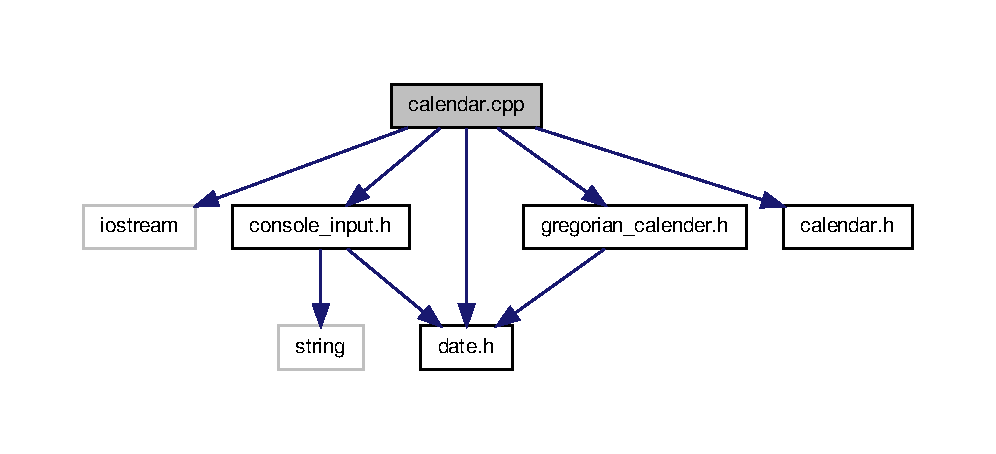
\includegraphics[width=350pt]{calendar_8cpp__incl}
\end{center}
\end{figure}
\subsection*{Functions}
\begin{DoxyCompactItemize}
\item 
void \hyperlink{calendar_8cpp_ad115f1168104746bd6f125391fbd0a99}{print\-\_\-actions} ()
\item 
void \hyperlink{calendar_8cpp_a395d2605875a0bf3296f56675c12edd7}{print\-\_\-goodbye} ()
\item 
void \hyperlink{calendar_8cpp_ab638c6fed68a7769bf26f7caecae3297}{generate\-\_\-and\-\_\-print\-\_\-calendar} ()
\item 
void \hyperlink{calendar_8cpp_a767223919a21b7a1054cbb8a3c543b76}{calc\-\_\-and\-\_\-print\-\_\-days\-\_\-between\-\_\-dates} ()
\end{DoxyCompactItemize}


\subsection{Function Documentation}
\hypertarget{calendar_8cpp_a767223919a21b7a1054cbb8a3c543b76}{\index{calendar.\-cpp@{calendar.\-cpp}!calc\-\_\-and\-\_\-print\-\_\-days\-\_\-between\-\_\-dates@{calc\-\_\-and\-\_\-print\-\_\-days\-\_\-between\-\_\-dates}}
\index{calc\-\_\-and\-\_\-print\-\_\-days\-\_\-between\-\_\-dates@{calc\-\_\-and\-\_\-print\-\_\-days\-\_\-between\-\_\-dates}!calendar.cpp@{calendar.\-cpp}}
\subsubsection[{calc\-\_\-and\-\_\-print\-\_\-days\-\_\-between\-\_\-dates}]{\setlength{\rightskip}{0pt plus 5cm}void calc\-\_\-and\-\_\-print\-\_\-days\-\_\-between\-\_\-dates (
\begin{DoxyParamCaption}
{}
\end{DoxyParamCaption}
)}}\label{calendar_8cpp_a767223919a21b7a1054cbb8a3c543b76}
Promts the user to enter two dates, calculates the days between them and prints the result to the console. 

Here is the call graph for this function\-:
\nopagebreak
\begin{figure}[H]
\begin{center}
\leavevmode
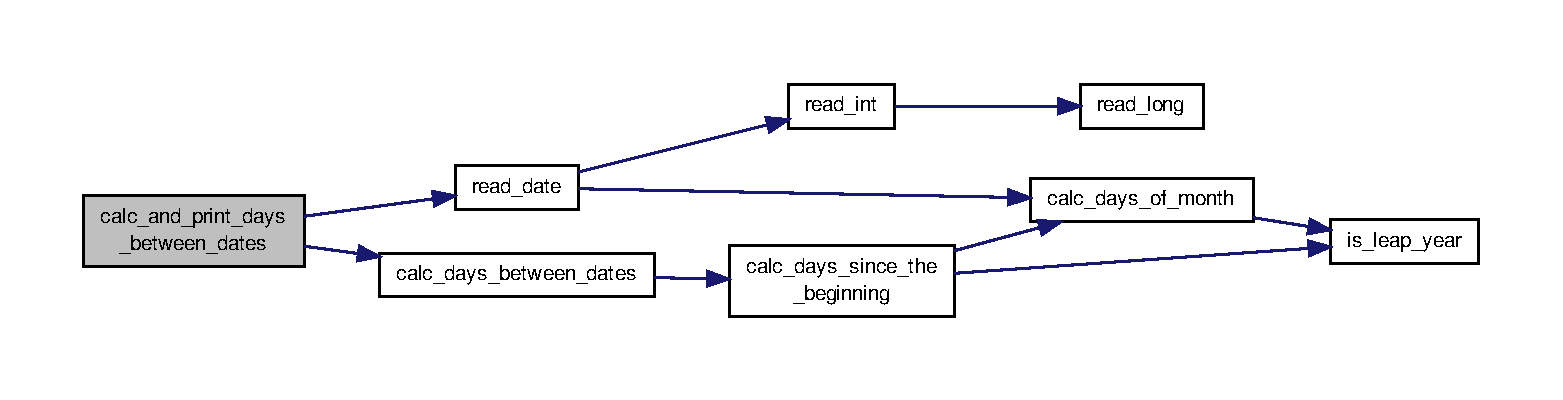
\includegraphics[width=350pt]{calendar_8cpp_a767223919a21b7a1054cbb8a3c543b76_cgraph}
\end{center}
\end{figure}


\hypertarget{calendar_8cpp_ab638c6fed68a7769bf26f7caecae3297}{\index{calendar.\-cpp@{calendar.\-cpp}!generate\-\_\-and\-\_\-print\-\_\-calendar@{generate\-\_\-and\-\_\-print\-\_\-calendar}}
\index{generate\-\_\-and\-\_\-print\-\_\-calendar@{generate\-\_\-and\-\_\-print\-\_\-calendar}!calendar.cpp@{calendar.\-cpp}}
\subsubsection[{generate\-\_\-and\-\_\-print\-\_\-calendar}]{\setlength{\rightskip}{0pt plus 5cm}void generate\-\_\-and\-\_\-print\-\_\-calendar (
\begin{DoxyParamCaption}
{}
\end{DoxyParamCaption}
)}}\label{calendar_8cpp_ab638c6fed68a7769bf26f7caecae3297}
Promts the user to enter a month of a year, and prints the according gregorian calender to the console. 

Here is the call graph for this function\-:
\nopagebreak
\begin{figure}[H]
\begin{center}
\leavevmode
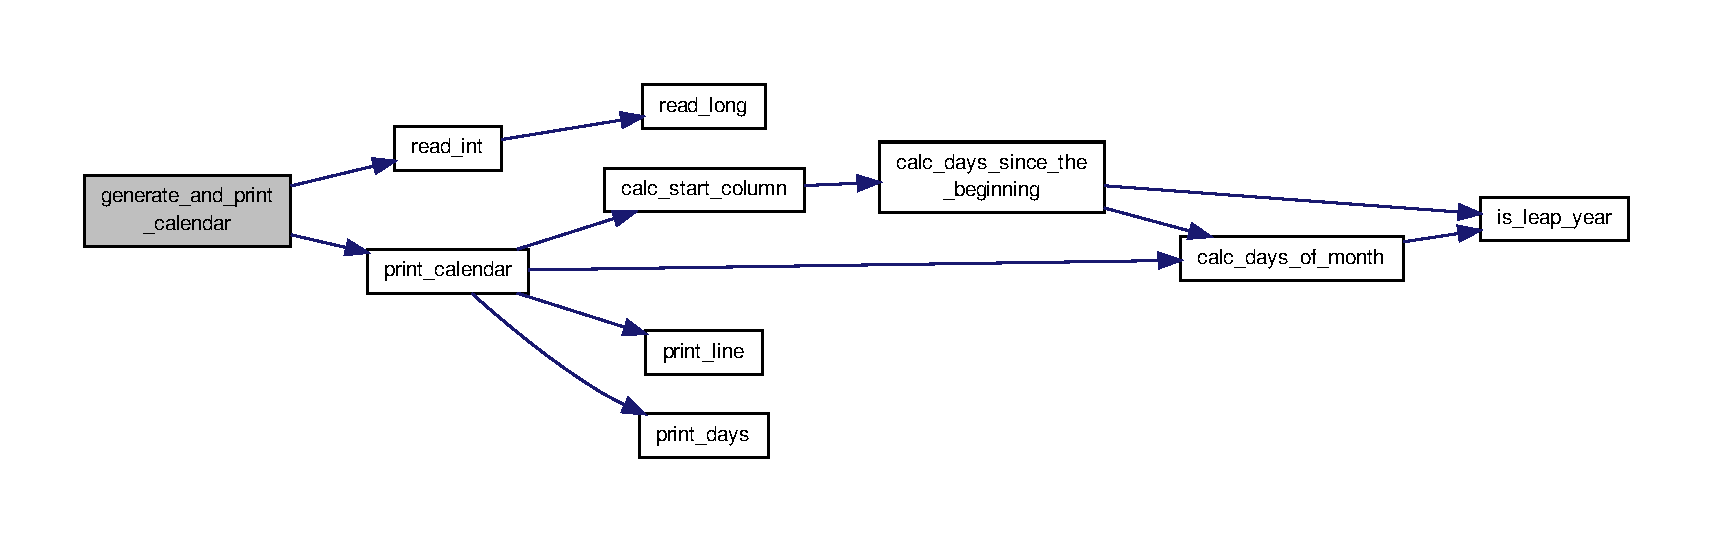
\includegraphics[width=350pt]{calendar_8cpp_ab638c6fed68a7769bf26f7caecae3297_cgraph}
\end{center}
\end{figure}


\hypertarget{calendar_8cpp_ad115f1168104746bd6f125391fbd0a99}{\index{calendar.\-cpp@{calendar.\-cpp}!print\-\_\-actions@{print\-\_\-actions}}
\index{print\-\_\-actions@{print\-\_\-actions}!calendar.cpp@{calendar.\-cpp}}
\subsubsection[{print\-\_\-actions}]{\setlength{\rightskip}{0pt plus 5cm}void print\-\_\-actions (
\begin{DoxyParamCaption}
{}
\end{DoxyParamCaption}
)}}\label{calendar_8cpp_ad115f1168104746bd6f125391fbd0a99}
Prints a description of the available actions to the console. \hypertarget{calendar_8cpp_a395d2605875a0bf3296f56675c12edd7}{\index{calendar.\-cpp@{calendar.\-cpp}!print\-\_\-goodbye@{print\-\_\-goodbye}}
\index{print\-\_\-goodbye@{print\-\_\-goodbye}!calendar.cpp@{calendar.\-cpp}}
\subsubsection[{print\-\_\-goodbye}]{\setlength{\rightskip}{0pt plus 5cm}void print\-\_\-goodbye (
\begin{DoxyParamCaption}
{}
\end{DoxyParamCaption}
)}}\label{calendar_8cpp_a395d2605875a0bf3296f56675c12edd7}
Prints a goodbye text to the console, when the program ends. 
\hypertarget{calendar_8h}{\section{calendar.\-h File Reference}
\label{calendar_8h}\index{calendar.\-h@{calendar.\-h}}
}
This graph shows which files directly or indirectly include this file\-:
\nopagebreak
\begin{figure}[H]
\begin{center}
\leavevmode
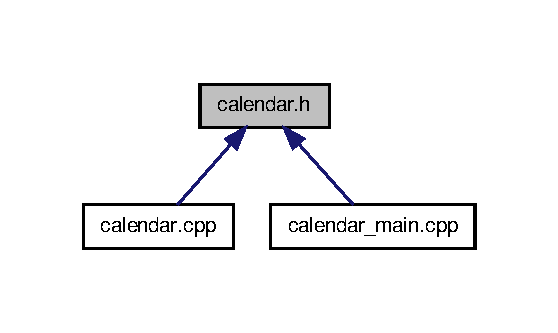
\includegraphics[width=176pt]{calendar_8h__dep__incl}
\end{center}
\end{figure}
\subsection*{Functions}
\begin{DoxyCompactItemize}
\item 
void \hyperlink{calendar_8h_ad115f1168104746bd6f125391fbd0a99}{print\-\_\-actions} ()
\item 
void \hyperlink{calendar_8h_a395d2605875a0bf3296f56675c12edd7}{print\-\_\-goodbye} ()
\item 
void \hyperlink{calendar_8h_ab638c6fed68a7769bf26f7caecae3297}{generate\-\_\-and\-\_\-print\-\_\-calendar} ()
\item 
void \hyperlink{calendar_8h_a767223919a21b7a1054cbb8a3c543b76}{calc\-\_\-and\-\_\-print\-\_\-days\-\_\-between\-\_\-dates} ()
\end{DoxyCompactItemize}


\subsection{Function Documentation}
\hypertarget{calendar_8h_a767223919a21b7a1054cbb8a3c543b76}{\index{calendar.\-h@{calendar.\-h}!calc\-\_\-and\-\_\-print\-\_\-days\-\_\-between\-\_\-dates@{calc\-\_\-and\-\_\-print\-\_\-days\-\_\-between\-\_\-dates}}
\index{calc\-\_\-and\-\_\-print\-\_\-days\-\_\-between\-\_\-dates@{calc\-\_\-and\-\_\-print\-\_\-days\-\_\-between\-\_\-dates}!calendar.h@{calendar.\-h}}
\subsubsection[{calc\-\_\-and\-\_\-print\-\_\-days\-\_\-between\-\_\-dates}]{\setlength{\rightskip}{0pt plus 5cm}void calc\-\_\-and\-\_\-print\-\_\-days\-\_\-between\-\_\-dates (
\begin{DoxyParamCaption}
{}
\end{DoxyParamCaption}
)}}\label{calendar_8h_a767223919a21b7a1054cbb8a3c543b76}
Promts the user to enter two dates, calculates the days between them and prints the result to the console. 

Here is the call graph for this function\-:
\nopagebreak
\begin{figure}[H]
\begin{center}
\leavevmode
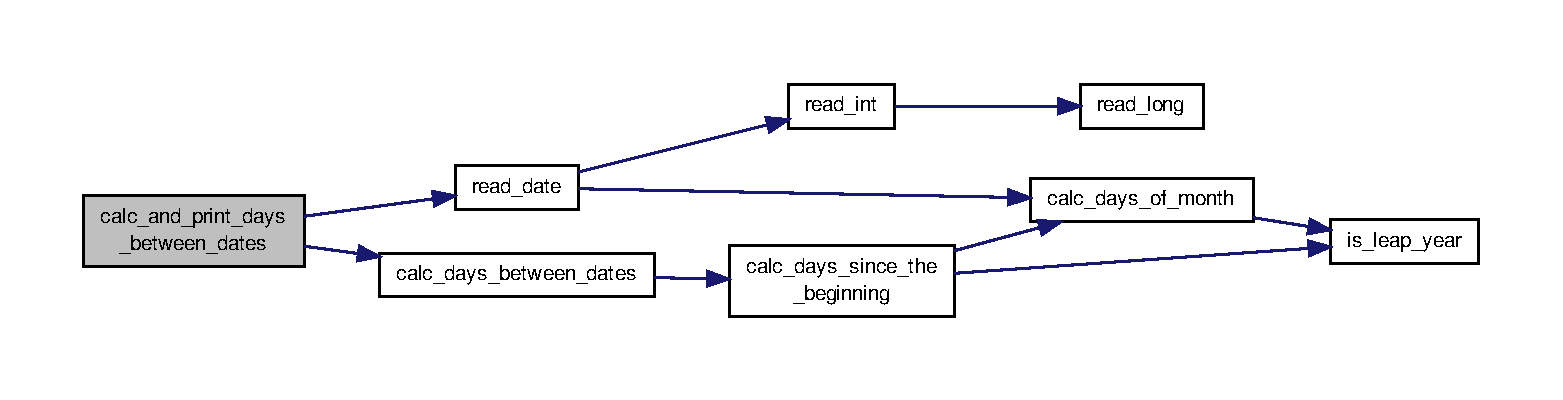
\includegraphics[width=350pt]{calendar_8h_a767223919a21b7a1054cbb8a3c543b76_cgraph}
\end{center}
\end{figure}


\hypertarget{calendar_8h_ab638c6fed68a7769bf26f7caecae3297}{\index{calendar.\-h@{calendar.\-h}!generate\-\_\-and\-\_\-print\-\_\-calendar@{generate\-\_\-and\-\_\-print\-\_\-calendar}}
\index{generate\-\_\-and\-\_\-print\-\_\-calendar@{generate\-\_\-and\-\_\-print\-\_\-calendar}!calendar.h@{calendar.\-h}}
\subsubsection[{generate\-\_\-and\-\_\-print\-\_\-calendar}]{\setlength{\rightskip}{0pt plus 5cm}void generate\-\_\-and\-\_\-print\-\_\-calendar (
\begin{DoxyParamCaption}
{}
\end{DoxyParamCaption}
)}}\label{calendar_8h_ab638c6fed68a7769bf26f7caecae3297}
Promts the user to enter a month of a year, and prints the according gregorian calender to the console. 

Here is the call graph for this function\-:
\nopagebreak
\begin{figure}[H]
\begin{center}
\leavevmode
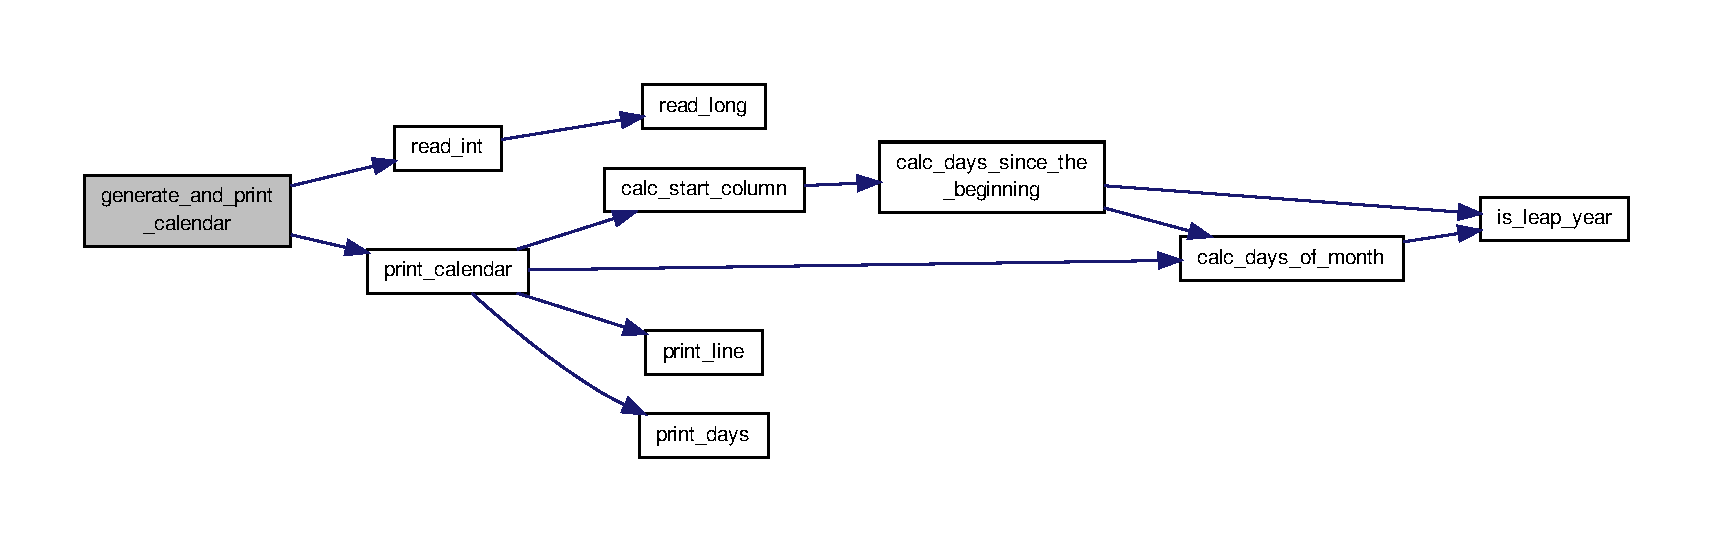
\includegraphics[width=350pt]{calendar_8h_ab638c6fed68a7769bf26f7caecae3297_cgraph}
\end{center}
\end{figure}


\hypertarget{calendar_8h_ad115f1168104746bd6f125391fbd0a99}{\index{calendar.\-h@{calendar.\-h}!print\-\_\-actions@{print\-\_\-actions}}
\index{print\-\_\-actions@{print\-\_\-actions}!calendar.h@{calendar.\-h}}
\subsubsection[{print\-\_\-actions}]{\setlength{\rightskip}{0pt plus 5cm}void print\-\_\-actions (
\begin{DoxyParamCaption}
{}
\end{DoxyParamCaption}
)}}\label{calendar_8h_ad115f1168104746bd6f125391fbd0a99}
Prints a description of the available actions to the console. \hypertarget{calendar_8h_a395d2605875a0bf3296f56675c12edd7}{\index{calendar.\-h@{calendar.\-h}!print\-\_\-goodbye@{print\-\_\-goodbye}}
\index{print\-\_\-goodbye@{print\-\_\-goodbye}!calendar.h@{calendar.\-h}}
\subsubsection[{print\-\_\-goodbye}]{\setlength{\rightskip}{0pt plus 5cm}void print\-\_\-goodbye (
\begin{DoxyParamCaption}
{}
\end{DoxyParamCaption}
)}}\label{calendar_8h_a395d2605875a0bf3296f56675c12edd7}
Prints a goodbye text to the console, when the program ends. 
\hypertarget{calendar__main_8cpp}{\section{calendar\-\_\-main.\-cpp File Reference}
\label{calendar__main_8cpp}\index{calendar\-\_\-main.\-cpp@{calendar\-\_\-main.\-cpp}}
}
{\ttfamily \#include \char`\"{}console\-\_\-input.\-h\char`\"{}}\\*
{\ttfamily \#include \char`\"{}calendar.\-h\char`\"{}}\\*
Include dependency graph for calendar\-\_\-main.\-cpp\-:
\nopagebreak
\begin{figure}[H]
\begin{center}
\leavevmode
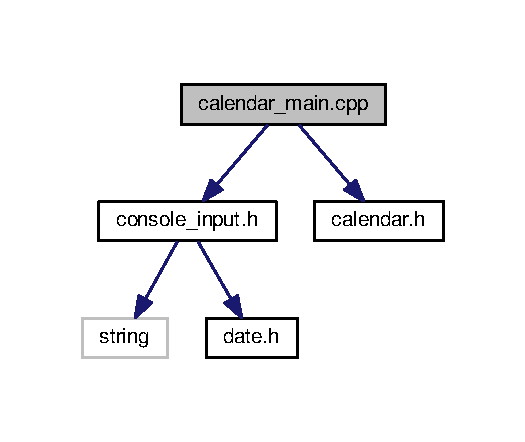
\includegraphics[width=252pt]{calendar__main_8cpp__incl}
\end{center}
\end{figure}
\subsection*{Functions}
\begin{DoxyCompactItemize}
\item 
int \hyperlink{calendar__main_8cpp_ae66f6b31b5ad750f1fe042a706a4e3d4}{main} ()
\end{DoxyCompactItemize}


\subsection{Function Documentation}
\hypertarget{calendar__main_8cpp_ae66f6b31b5ad750f1fe042a706a4e3d4}{\index{calendar\-\_\-main.\-cpp@{calendar\-\_\-main.\-cpp}!main@{main}}
\index{main@{main}!calendar_main.cpp@{calendar\-\_\-main.\-cpp}}
\subsubsection[{main}]{\setlength{\rightskip}{0pt plus 5cm}int main (
\begin{DoxyParamCaption}
{}
\end{DoxyParamCaption}
)}}\label{calendar__main_8cpp_ae66f6b31b5ad750f1fe042a706a4e3d4}
Entrypoint for the calendar application. It includes three different action.
\begin{DoxyEnumerate}
\item Create a calendar for a any month of a year between 1583 and 1000000.
\item Calculates days between two arbitary dates.
\item End of the program.
\end{DoxyEnumerate}

It uses the gregorian calendar und is aware of leap years. The user entry is validated, so that it is not possible to enter a wrong date e.\-g. 30.\-02.\-2004 or 29.\-02.\-2014. 

Here is the call graph for this function\-:
\nopagebreak
\begin{figure}[H]
\begin{center}
\leavevmode
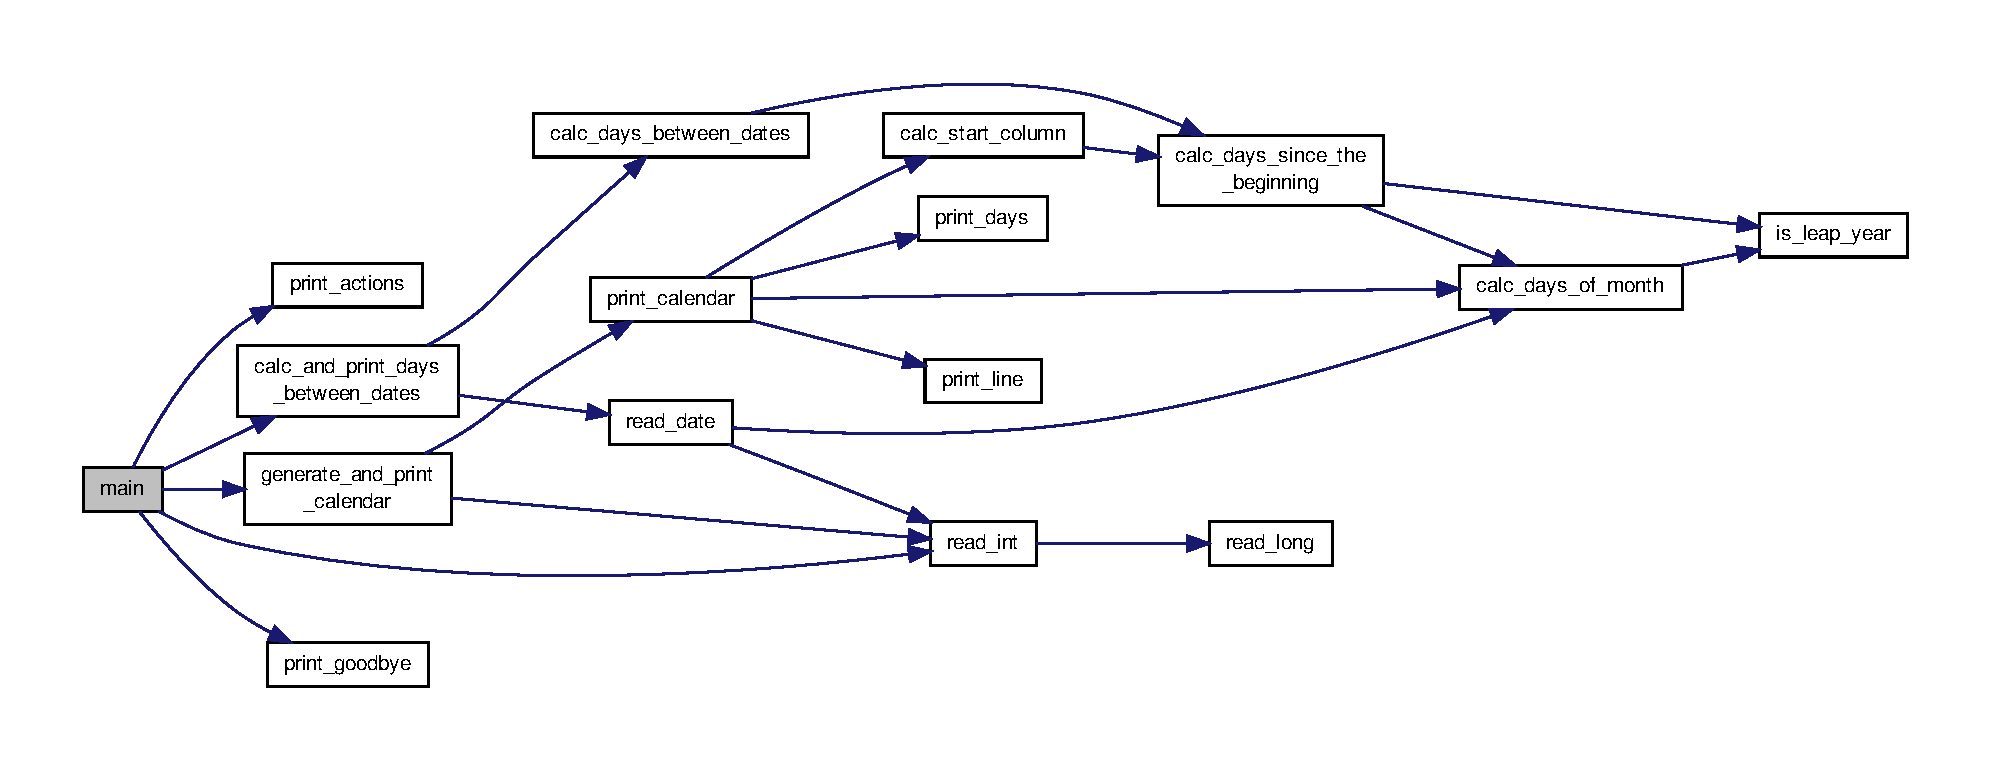
\includegraphics[width=350pt]{calendar__main_8cpp_ae66f6b31b5ad750f1fe042a706a4e3d4_cgraph}
\end{center}
\end{figure}



\hypertarget{console__input_8cpp}{\section{console\-\_\-input.\-cpp File Reference}
\label{console__input_8cpp}\index{console\-\_\-input.\-cpp@{console\-\_\-input.\-cpp}}
}
{\ttfamily \#include $<$iostream$>$}\\*
{\ttfamily \#include $<$limits$>$}\\*
{\ttfamily \#include $<$string$>$}\\*
{\ttfamily \#include \char`\"{}console\-\_\-input.\-h\char`\"{}}\\*
Include dependency graph for console\-\_\-input.\-cpp\-:\nopagebreak
\begin{figure}[H]
\begin{center}
\leavevmode
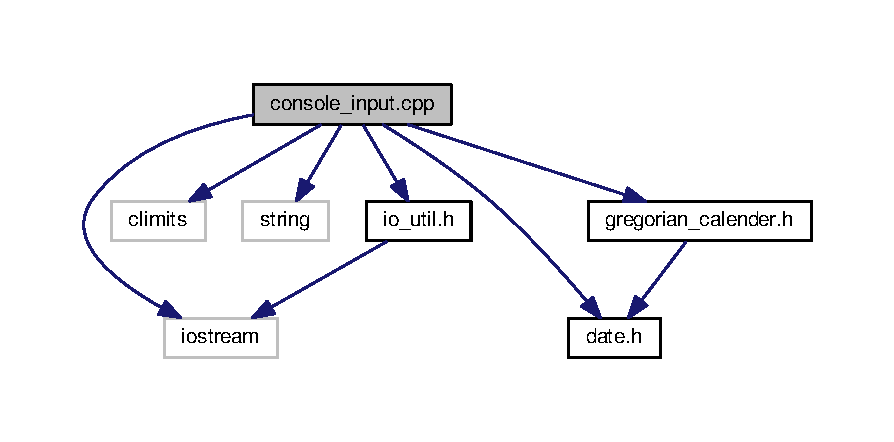
\includegraphics[width=332pt]{console__input_8cpp__incl}
\end{center}
\end{figure}
\subsection*{Functions}
\begin{DoxyCompactItemize}
\item 
double \hyperlink{console__input_8cpp_a8a9df77c5c4adba7ebadb77f3b3dc8ee}{read\-\_\-double} (double min, double max)
\item 
double \hyperlink{console__input_8cpp_a65f2421973540c10e5ae7d10177c566a}{read\-\_\-double} ()
\item 
double \hyperlink{console__input_8cpp_a46878a8594ba71f54911c572031d4614}{read\-\_\-double} (string text)
\item 
double \hyperlink{console__input_8cpp_aca43573be8fe10d4bfede3fc5bd0bd63}{read\-\_\-double} (string text, double min, double max)
\item 
long \hyperlink{console__input_8cpp_a710a686867142de265860584f4147592}{read\-\_\-long} (long min, long max)
\item 
long \hyperlink{console__input_8cpp_a347c616893b725a74f60ea1f7ee325d2}{read\-\_\-long} ()
\item 
long \hyperlink{console__input_8cpp_a9128c63513d87af5259597d8c9930476}{read\-\_\-long} (string text)
\item 
long \hyperlink{console__input_8cpp_a03ebbd2a45117ee03be4e9002210ab36}{read\-\_\-long} (string text, long min, long max)
\item 
int \hyperlink{console__input_8cpp_ad0ccfbb50d0e333ef8acfeab2b7d8071}{read\-\_\-int} (int min, int max)
\item 
int \hyperlink{console__input_8cpp_af310540093ee953c3018bc13bbde3da5}{read\-\_\-int} ()
\item 
int \hyperlink{console__input_8cpp_aaaf3786f6b4803f3120609011de4b0db}{read\-\_\-int} (string text)
\item 
int \hyperlink{console__input_8cpp_a4f8c1bb51d432116d3eda43db3340c8c}{read\-\_\-int} (string text, int min, int max)
\item 
bool \hyperlink{console__input_8cpp_a6bac3909a28fff2736a171022343380b}{read\-\_\-yes\-\_\-no} (string text)
\item 
string \hyperlink{console__input_8cpp_a44ccadd65be527f89bdcf6d27a3b1147}{read\-\_\-text} (string text)
\end{DoxyCompactItemize}


\subsection{Function Documentation}
\hypertarget{console__input_8cpp_a8a9df77c5c4adba7ebadb77f3b3dc8ee}{\index{console\-\_\-input.\-cpp@{console\-\_\-input.\-cpp}!read\-\_\-double@{read\-\_\-double}}
\index{read\-\_\-double@{read\-\_\-double}!console_input.cpp@{console\-\_\-input.\-cpp}}
\subsubsection[{read\-\_\-double}]{\setlength{\rightskip}{0pt plus 5cm}double read\-\_\-double (
\begin{DoxyParamCaption}
\item[{double}]{min, }
\item[{double}]{max}
\end{DoxyParamCaption}
)}}\label{console__input_8cpp_a8a9df77c5c4adba7ebadb77f3b3dc8ee}
Reads a double value in between a given interval from the console. When the entered value is not valid to the interval, the user gets prompted to reenter a valid.


\begin{DoxyParams}{Parameters}
{\em min} & lower bound of the interval. \\
\hline
{\em max} & top bound of the interval\\
\hline
\end{DoxyParams}
\begin{DoxyReturn}{Returns}
a double value in between min and max. 
\end{DoxyReturn}
\hypertarget{console__input_8cpp_a65f2421973540c10e5ae7d10177c566a}{\index{console\-\_\-input.\-cpp@{console\-\_\-input.\-cpp}!read\-\_\-double@{read\-\_\-double}}
\index{read\-\_\-double@{read\-\_\-double}!console_input.cpp@{console\-\_\-input.\-cpp}}
\subsubsection[{read\-\_\-double}]{\setlength{\rightskip}{0pt plus 5cm}double read\-\_\-double (
\begin{DoxyParamCaption}
{}
\end{DoxyParamCaption}
)}}\label{console__input_8cpp_a65f2421973540c10e5ae7d10177c566a}
Reads a double value from the console in between the whole range of double.

\begin{DoxyReturn}{Returns}
a valid double value. 
\end{DoxyReturn}


Here is the call graph for this function\-:\nopagebreak
\begin{figure}[H]
\begin{center}
\leavevmode
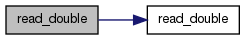
\includegraphics[width=256pt]{console__input_8cpp_a65f2421973540c10e5ae7d10177c566a_cgraph}
\end{center}
\end{figure}


\hypertarget{console__input_8cpp_a46878a8594ba71f54911c572031d4614}{\index{console\-\_\-input.\-cpp@{console\-\_\-input.\-cpp}!read\-\_\-double@{read\-\_\-double}}
\index{read\-\_\-double@{read\-\_\-double}!console_input.cpp@{console\-\_\-input.\-cpp}}
\subsubsection[{read\-\_\-double}]{\setlength{\rightskip}{0pt plus 5cm}double read\-\_\-double (
\begin{DoxyParamCaption}
\item[{string}]{text}
\end{DoxyParamCaption}
)}}\label{console__input_8cpp_a46878a8594ba71f54911c572031d4614}
Prints a text to the console and reads a double value from the console in between the whole range of double.


\begin{DoxyParams}{Parameters}
{\em text} & text to print to the console.\\
\hline
\end{DoxyParams}
\begin{DoxyReturn}{Returns}
a valid double value. 
\end{DoxyReturn}


Here is the call graph for this function\-:\nopagebreak
\begin{figure}[H]
\begin{center}
\leavevmode
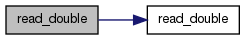
\includegraphics[width=256pt]{console__input_8cpp_a46878a8594ba71f54911c572031d4614_cgraph}
\end{center}
\end{figure}


\hypertarget{console__input_8cpp_aca43573be8fe10d4bfede3fc5bd0bd63}{\index{console\-\_\-input.\-cpp@{console\-\_\-input.\-cpp}!read\-\_\-double@{read\-\_\-double}}
\index{read\-\_\-double@{read\-\_\-double}!console_input.cpp@{console\-\_\-input.\-cpp}}
\subsubsection[{read\-\_\-double}]{\setlength{\rightskip}{0pt plus 5cm}double read\-\_\-double (
\begin{DoxyParamCaption}
\item[{string}]{text, }
\item[{double}]{min, }
\item[{double}]{max}
\end{DoxyParamCaption}
)}}\label{console__input_8cpp_aca43573be8fe10d4bfede3fc5bd0bd63}


Here is the call graph for this function\-:\nopagebreak
\begin{figure}[H]
\begin{center}
\leavevmode
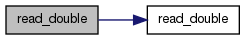
\includegraphics[width=256pt]{console__input_8cpp_aca43573be8fe10d4bfede3fc5bd0bd63_cgraph}
\end{center}
\end{figure}


\hypertarget{console__input_8cpp_ad0ccfbb50d0e333ef8acfeab2b7d8071}{\index{console\-\_\-input.\-cpp@{console\-\_\-input.\-cpp}!read\-\_\-int@{read\-\_\-int}}
\index{read\-\_\-int@{read\-\_\-int}!console_input.cpp@{console\-\_\-input.\-cpp}}
\subsubsection[{read\-\_\-int}]{\setlength{\rightskip}{0pt plus 5cm}int read\-\_\-int (
\begin{DoxyParamCaption}
\item[{int}]{min, }
\item[{int}]{max}
\end{DoxyParamCaption}
)}}\label{console__input_8cpp_ad0ccfbb50d0e333ef8acfeab2b7d8071}
Reads a integer value in between a given interval from the console. When the entered value is not valid to the interval, the user gets prompted to reenter a valid.


\begin{DoxyParams}{Parameters}
{\em min} & lower bound of the interval. \\
\hline
{\em max} & top bound of the interval\\
\hline
\end{DoxyParams}
\begin{DoxyReturn}{Returns}
a int value in between min and max. 
\end{DoxyReturn}


Here is the call graph for this function\-:\nopagebreak
\begin{figure}[H]
\begin{center}
\leavevmode
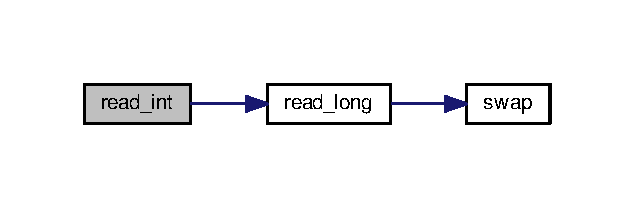
\includegraphics[width=334pt]{console__input_8cpp_ad0ccfbb50d0e333ef8acfeab2b7d8071_cgraph}
\end{center}
\end{figure}


\hypertarget{console__input_8cpp_af310540093ee953c3018bc13bbde3da5}{\index{console\-\_\-input.\-cpp@{console\-\_\-input.\-cpp}!read\-\_\-int@{read\-\_\-int}}
\index{read\-\_\-int@{read\-\_\-int}!console_input.cpp@{console\-\_\-input.\-cpp}}
\subsubsection[{read\-\_\-int}]{\setlength{\rightskip}{0pt plus 5cm}int read\-\_\-int (
\begin{DoxyParamCaption}
{}
\end{DoxyParamCaption}
)}}\label{console__input_8cpp_af310540093ee953c3018bc13bbde3da5}
Reads an integer value from the terminal in between the whole range of long.

\begin{DoxyReturn}{Returns}
a valid integer value. 
\end{DoxyReturn}


Here is the call graph for this function\-:\nopagebreak
\begin{figure}[H]
\begin{center}
\leavevmode
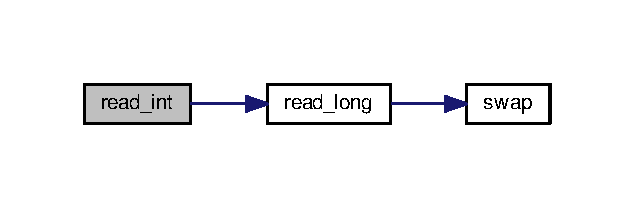
\includegraphics[width=334pt]{console__input_8cpp_af310540093ee953c3018bc13bbde3da5_cgraph}
\end{center}
\end{figure}


\hypertarget{console__input_8cpp_aaaf3786f6b4803f3120609011de4b0db}{\index{console\-\_\-input.\-cpp@{console\-\_\-input.\-cpp}!read\-\_\-int@{read\-\_\-int}}
\index{read\-\_\-int@{read\-\_\-int}!console_input.cpp@{console\-\_\-input.\-cpp}}
\subsubsection[{read\-\_\-int}]{\setlength{\rightskip}{0pt plus 5cm}int read\-\_\-int (
\begin{DoxyParamCaption}
\item[{string}]{text}
\end{DoxyParamCaption}
)}}\label{console__input_8cpp_aaaf3786f6b4803f3120609011de4b0db}
Prints a text to the console and reads a integer value from the console in between the whole range of integer.


\begin{DoxyParams}{Parameters}
{\em text} & text to print to the console.\\
\hline
\end{DoxyParams}
\begin{DoxyReturn}{Returns}
a valid integer value. 
\end{DoxyReturn}


Here is the call graph for this function\-:\nopagebreak
\begin{figure}[H]
\begin{center}
\leavevmode
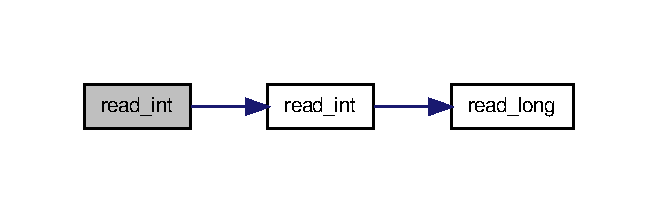
\includegraphics[width=350pt]{console__input_8cpp_aaaf3786f6b4803f3120609011de4b0db_cgraph}
\end{center}
\end{figure}


\hypertarget{console__input_8cpp_a4f8c1bb51d432116d3eda43db3340c8c}{\index{console\-\_\-input.\-cpp@{console\-\_\-input.\-cpp}!read\-\_\-int@{read\-\_\-int}}
\index{read\-\_\-int@{read\-\_\-int}!console_input.cpp@{console\-\_\-input.\-cpp}}
\subsubsection[{read\-\_\-int}]{\setlength{\rightskip}{0pt plus 5cm}int read\-\_\-int (
\begin{DoxyParamCaption}
\item[{string}]{text, }
\item[{int}]{min, }
\item[{int}]{max}
\end{DoxyParamCaption}
)}}\label{console__input_8cpp_a4f8c1bb51d432116d3eda43db3340c8c}
Prints a text to the console and reads a integer value in between a given interval from the console. When the value is not in between the interval, the user gets prompted to reeinter a valid value.


\begin{DoxyParams}{Parameters}
{\em text} & text to print to the console. \\
\hline
{\em min} & lower bound of the interval. \\
\hline
{\em max} & top bound of the interval.\\
\hline
\end{DoxyParams}
\begin{DoxyReturn}{Returns}
a integer value in between min and max. 
\end{DoxyReturn}


Here is the call graph for this function\-:\nopagebreak
\begin{figure}[H]
\begin{center}
\leavevmode
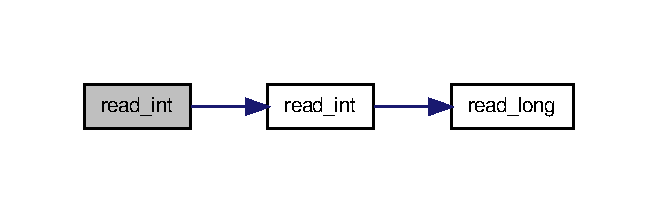
\includegraphics[width=350pt]{console__input_8cpp_a4f8c1bb51d432116d3eda43db3340c8c_cgraph}
\end{center}
\end{figure}


\hypertarget{console__input_8cpp_a710a686867142de265860584f4147592}{\index{console\-\_\-input.\-cpp@{console\-\_\-input.\-cpp}!read\-\_\-long@{read\-\_\-long}}
\index{read\-\_\-long@{read\-\_\-long}!console_input.cpp@{console\-\_\-input.\-cpp}}
\subsubsection[{read\-\_\-long}]{\setlength{\rightskip}{0pt plus 5cm}long read\-\_\-long (
\begin{DoxyParamCaption}
\item[{long}]{min, }
\item[{long}]{max}
\end{DoxyParamCaption}
)}}\label{console__input_8cpp_a710a686867142de265860584f4147592}
Reads a long value in between a given interval from the console. When the entered value is not valid to the interval, the user gets prompted to reenter a valid.


\begin{DoxyParams}{Parameters}
{\em min} & lower bound of the interval. \\
\hline
{\em max} & top bound of the interval\\
\hline
\end{DoxyParams}
\begin{DoxyReturn}{Returns}
a long value in between min and max. 
\end{DoxyReturn}


Here is the call graph for this function\-:\nopagebreak
\begin{figure}[H]
\begin{center}
\leavevmode
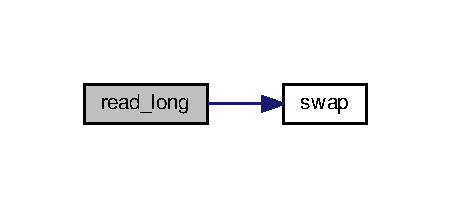
\includegraphics[width=246pt]{console__input_8cpp_a710a686867142de265860584f4147592_cgraph}
\end{center}
\end{figure}


\hypertarget{console__input_8cpp_a347c616893b725a74f60ea1f7ee325d2}{\index{console\-\_\-input.\-cpp@{console\-\_\-input.\-cpp}!read\-\_\-long@{read\-\_\-long}}
\index{read\-\_\-long@{read\-\_\-long}!console_input.cpp@{console\-\_\-input.\-cpp}}
\subsubsection[{read\-\_\-long}]{\setlength{\rightskip}{0pt plus 5cm}long read\-\_\-long (
\begin{DoxyParamCaption}
{}
\end{DoxyParamCaption}
)}}\label{console__input_8cpp_a347c616893b725a74f60ea1f7ee325d2}
Reads a long value from the terminal in between the whole range of long.

\begin{DoxyReturn}{Returns}
a valid long value. 
\end{DoxyReturn}


Here is the call graph for this function\-:\nopagebreak
\begin{figure}[H]
\begin{center}
\leavevmode
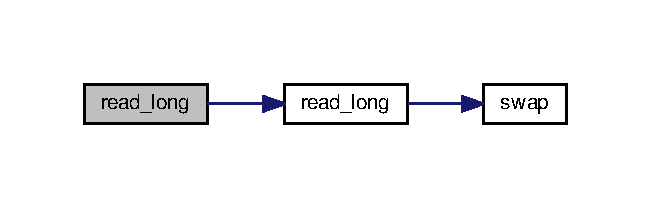
\includegraphics[width=342pt]{console__input_8cpp_a347c616893b725a74f60ea1f7ee325d2_cgraph}
\end{center}
\end{figure}


\hypertarget{console__input_8cpp_a9128c63513d87af5259597d8c9930476}{\index{console\-\_\-input.\-cpp@{console\-\_\-input.\-cpp}!read\-\_\-long@{read\-\_\-long}}
\index{read\-\_\-long@{read\-\_\-long}!console_input.cpp@{console\-\_\-input.\-cpp}}
\subsubsection[{read\-\_\-long}]{\setlength{\rightskip}{0pt plus 5cm}long read\-\_\-long (
\begin{DoxyParamCaption}
\item[{string}]{text}
\end{DoxyParamCaption}
)}}\label{console__input_8cpp_a9128c63513d87af5259597d8c9930476}
Prints a text to the console and reads a long value from the console in between the whole range of long.


\begin{DoxyParams}{Parameters}
{\em text} & text to print to the console.\\
\hline
\end{DoxyParams}
\begin{DoxyReturn}{Returns}
a valid long value. 
\end{DoxyReturn}


Here is the call graph for this function\-:\nopagebreak
\begin{figure}[H]
\begin{center}
\leavevmode
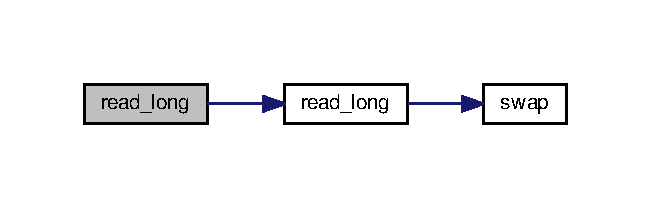
\includegraphics[width=342pt]{console__input_8cpp_a9128c63513d87af5259597d8c9930476_cgraph}
\end{center}
\end{figure}


\hypertarget{console__input_8cpp_a03ebbd2a45117ee03be4e9002210ab36}{\index{console\-\_\-input.\-cpp@{console\-\_\-input.\-cpp}!read\-\_\-long@{read\-\_\-long}}
\index{read\-\_\-long@{read\-\_\-long}!console_input.cpp@{console\-\_\-input.\-cpp}}
\subsubsection[{read\-\_\-long}]{\setlength{\rightskip}{0pt plus 5cm}long read\-\_\-long (
\begin{DoxyParamCaption}
\item[{string}]{text, }
\item[{long}]{min, }
\item[{long}]{max}
\end{DoxyParamCaption}
)}}\label{console__input_8cpp_a03ebbd2a45117ee03be4e9002210ab36}
Prints a text to the console and reads a long value in between a given interval from the console. When the value is not in between the interval, the user gets prompted to reeinter a valid value.


\begin{DoxyParams}{Parameters}
{\em text} & text to print to the console. \\
\hline
{\em min} & lower bound of the interval. \\
\hline
{\em max} & top bound of the interval.\\
\hline
\end{DoxyParams}
\begin{DoxyReturn}{Returns}
a long value in between min and max. 
\end{DoxyReturn}


Here is the call graph for this function\-:\nopagebreak
\begin{figure}[H]
\begin{center}
\leavevmode
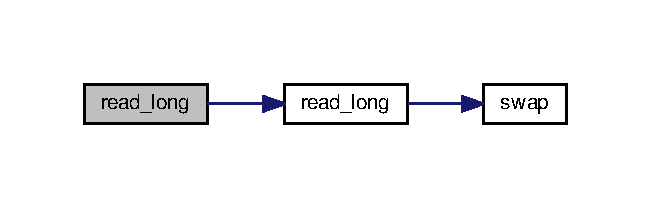
\includegraphics[width=342pt]{console__input_8cpp_a03ebbd2a45117ee03be4e9002210ab36_cgraph}
\end{center}
\end{figure}


\hypertarget{console__input_8cpp_a44ccadd65be527f89bdcf6d27a3b1147}{\index{console\-\_\-input.\-cpp@{console\-\_\-input.\-cpp}!read\-\_\-text@{read\-\_\-text}}
\index{read\-\_\-text@{read\-\_\-text}!console_input.cpp@{console\-\_\-input.\-cpp}}
\subsubsection[{read\-\_\-text}]{\setlength{\rightskip}{0pt plus 5cm}string read\-\_\-text (
\begin{DoxyParamCaption}
\item[{string}]{text}
\end{DoxyParamCaption}
)}}\label{console__input_8cpp_a44ccadd65be527f89bdcf6d27a3b1147}
\hypertarget{console__input_8cpp_a6bac3909a28fff2736a171022343380b}{\index{console\-\_\-input.\-cpp@{console\-\_\-input.\-cpp}!read\-\_\-yes\-\_\-no@{read\-\_\-yes\-\_\-no}}
\index{read\-\_\-yes\-\_\-no@{read\-\_\-yes\-\_\-no}!console_input.cpp@{console\-\_\-input.\-cpp}}
\subsubsection[{read\-\_\-yes\-\_\-no}]{\setlength{\rightskip}{0pt plus 5cm}bool read\-\_\-yes\-\_\-no (
\begin{DoxyParamCaption}
\item[{string}]{text}
\end{DoxyParamCaption}
)}}\label{console__input_8cpp_a6bac3909a28fff2736a171022343380b}

\hypertarget{console__input_8h}{\section{console\-\_\-input.\-h File Reference}
\label{console__input_8h}\index{console\-\_\-input.\-h@{console\-\_\-input.\-h}}
}
{\ttfamily \#include $<$string$>$}\\*
Include dependency graph for console\-\_\-input.\-h\-:\nopagebreak
\begin{figure}[H]
\begin{center}
\leavevmode
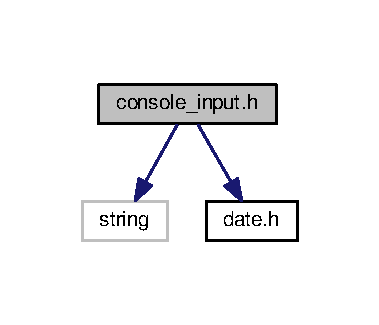
\includegraphics[width=164pt]{console__input_8h__incl}
\end{center}
\end{figure}
This graph shows which files directly or indirectly include this file\-:\nopagebreak
\begin{figure}[H]
\begin{center}
\leavevmode
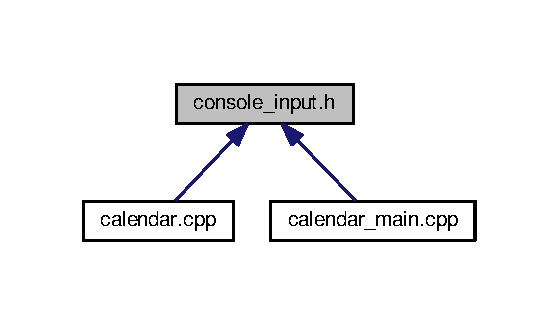
\includegraphics[width=264pt]{console__input_8h__dep__incl}
\end{center}
\end{figure}
\subsection*{Functions}
\begin{DoxyCompactItemize}
\item 
double \hyperlink{console__input_8h_a8a9df77c5c4adba7ebadb77f3b3dc8ee}{read\-\_\-double} (double min, double max)
\item 
double \hyperlink{console__input_8h_a46878a8594ba71f54911c572031d4614}{read\-\_\-double} (string text)
\item 
double \hyperlink{console__input_8h_aca43573be8fe10d4bfede3fc5bd0bd63}{read\-\_\-double} (string text, double min, double max)
\item 
double \hyperlink{console__input_8h_a65f2421973540c10e5ae7d10177c566a}{read\-\_\-double} ()
\item 
void \hyperlink{console__input_8h_afc6e4adf69aec96a5eae4249fbbc7201}{read\-\_\-enter} ()
\item 
long \hyperlink{console__input_8h_a03ebbd2a45117ee03be4e9002210ab36}{read\-\_\-long} (string text, long min, long max)
\item 
long \hyperlink{console__input_8h_a710a686867142de265860584f4147592}{read\-\_\-long} (long min, long max)
\item 
long \hyperlink{console__input_8h_a9128c63513d87af5259597d8c9930476}{read\-\_\-long} (string text)
\item 
long \hyperlink{console__input_8h_a347c616893b725a74f60ea1f7ee325d2}{read\-\_\-long} ()
\item 
int \hyperlink{console__input_8h_a4f8c1bb51d432116d3eda43db3340c8c}{read\-\_\-int} (string text, int min, int max)
\item 
int \hyperlink{console__input_8h_ad0ccfbb50d0e333ef8acfeab2b7d8071}{read\-\_\-int} (int min, int max)
\item 
int \hyperlink{console__input_8h_aaaf3786f6b4803f3120609011de4b0db}{read\-\_\-int} (string text)
\item 
int \hyperlink{console__input_8h_af310540093ee953c3018bc13bbde3da5}{read\-\_\-int} ()
\item 
bool \hyperlink{console__input_8h_a6bac3909a28fff2736a171022343380b}{read\-\_\-yes\-\_\-no} (string text)
\item 
string \hyperlink{console__input_8h_a44ccadd65be527f89bdcf6d27a3b1147}{read\-\_\-text} (string text)
\end{DoxyCompactItemize}


\subsection{Function Documentation}
\hypertarget{console__input_8h_a8a9df77c5c4adba7ebadb77f3b3dc8ee}{\index{console\-\_\-input.\-h@{console\-\_\-input.\-h}!read\-\_\-double@{read\-\_\-double}}
\index{read\-\_\-double@{read\-\_\-double}!console_input.h@{console\-\_\-input.\-h}}
\subsubsection[{read\-\_\-double}]{\setlength{\rightskip}{0pt plus 5cm}double read\-\_\-double (
\begin{DoxyParamCaption}
\item[{double}]{min, }
\item[{double}]{max}
\end{DoxyParamCaption}
)}}\label{console__input_8h_a8a9df77c5c4adba7ebadb77f3b3dc8ee}
Reads a double value in between a given interval from the console. When the entered value is not valid to the interval, the user gets prompted to reenter a valid.


\begin{DoxyParams}{Parameters}
{\em min} & lower bound of the interval. \\
\hline
{\em max} & top bound of the interval\\
\hline
\end{DoxyParams}
\begin{DoxyReturn}{Returns}
a double value in between min and max. 
\end{DoxyReturn}
\hypertarget{console__input_8h_a46878a8594ba71f54911c572031d4614}{\index{console\-\_\-input.\-h@{console\-\_\-input.\-h}!read\-\_\-double@{read\-\_\-double}}
\index{read\-\_\-double@{read\-\_\-double}!console_input.h@{console\-\_\-input.\-h}}
\subsubsection[{read\-\_\-double}]{\setlength{\rightskip}{0pt plus 5cm}double read\-\_\-double (
\begin{DoxyParamCaption}
\item[{string}]{text}
\end{DoxyParamCaption}
)}}\label{console__input_8h_a46878a8594ba71f54911c572031d4614}
Prints a text to the console and reads a double value from the console in between the whole range of double.


\begin{DoxyParams}{Parameters}
{\em text} & text to print to the console.\\
\hline
\end{DoxyParams}
\begin{DoxyReturn}{Returns}
a valid double value. 
\end{DoxyReturn}


Here is the call graph for this function\-:\nopagebreak
\begin{figure}[H]
\begin{center}
\leavevmode
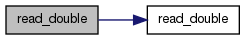
\includegraphics[width=256pt]{console__input_8h_a46878a8594ba71f54911c572031d4614_cgraph}
\end{center}
\end{figure}


\hypertarget{console__input_8h_aca43573be8fe10d4bfede3fc5bd0bd63}{\index{console\-\_\-input.\-h@{console\-\_\-input.\-h}!read\-\_\-double@{read\-\_\-double}}
\index{read\-\_\-double@{read\-\_\-double}!console_input.h@{console\-\_\-input.\-h}}
\subsubsection[{read\-\_\-double}]{\setlength{\rightskip}{0pt plus 5cm}double read\-\_\-double (
\begin{DoxyParamCaption}
\item[{string}]{text, }
\item[{double}]{min, }
\item[{double}]{max}
\end{DoxyParamCaption}
)}}\label{console__input_8h_aca43573be8fe10d4bfede3fc5bd0bd63}


Here is the call graph for this function\-:\nopagebreak
\begin{figure}[H]
\begin{center}
\leavevmode
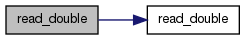
\includegraphics[width=256pt]{console__input_8h_aca43573be8fe10d4bfede3fc5bd0bd63_cgraph}
\end{center}
\end{figure}


\hypertarget{console__input_8h_a65f2421973540c10e5ae7d10177c566a}{\index{console\-\_\-input.\-h@{console\-\_\-input.\-h}!read\-\_\-double@{read\-\_\-double}}
\index{read\-\_\-double@{read\-\_\-double}!console_input.h@{console\-\_\-input.\-h}}
\subsubsection[{read\-\_\-double}]{\setlength{\rightskip}{0pt plus 5cm}double read\-\_\-double (
\begin{DoxyParamCaption}
{}
\end{DoxyParamCaption}
)}}\label{console__input_8h_a65f2421973540c10e5ae7d10177c566a}
Reads a double value from the console in between the whole range of double.

\begin{DoxyReturn}{Returns}
a valid double value. 
\end{DoxyReturn}


Here is the call graph for this function\-:\nopagebreak
\begin{figure}[H]
\begin{center}
\leavevmode
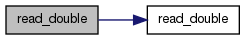
\includegraphics[width=256pt]{console__input_8h_a65f2421973540c10e5ae7d10177c566a_cgraph}
\end{center}
\end{figure}


\hypertarget{console__input_8h_afc6e4adf69aec96a5eae4249fbbc7201}{\index{console\-\_\-input.\-h@{console\-\_\-input.\-h}!read\-\_\-enter@{read\-\_\-enter}}
\index{read\-\_\-enter@{read\-\_\-enter}!console_input.h@{console\-\_\-input.\-h}}
\subsubsection[{read\-\_\-enter}]{\setlength{\rightskip}{0pt plus 5cm}void read\-\_\-enter (
\begin{DoxyParamCaption}
{}
\end{DoxyParamCaption}
)}}\label{console__input_8h_afc6e4adf69aec96a5eae4249fbbc7201}
\hypertarget{console__input_8h_a4f8c1bb51d432116d3eda43db3340c8c}{\index{console\-\_\-input.\-h@{console\-\_\-input.\-h}!read\-\_\-int@{read\-\_\-int}}
\index{read\-\_\-int@{read\-\_\-int}!console_input.h@{console\-\_\-input.\-h}}
\subsubsection[{read\-\_\-int}]{\setlength{\rightskip}{0pt plus 5cm}int read\-\_\-int (
\begin{DoxyParamCaption}
\item[{string}]{text, }
\item[{int}]{min, }
\item[{int}]{max}
\end{DoxyParamCaption}
)}}\label{console__input_8h_a4f8c1bb51d432116d3eda43db3340c8c}
Prints a text to the console and reads a integer value in between a given interval from the console. When the value is not in between the interval, the user gets prompted to reeinter a valid value.


\begin{DoxyParams}{Parameters}
{\em text} & text to print to the console. \\
\hline
{\em min} & lower bound of the interval. \\
\hline
{\em max} & top bound of the interval.\\
\hline
\end{DoxyParams}
\begin{DoxyReturn}{Returns}
a integer value in between min and max. 
\end{DoxyReturn}


Here is the call graph for this function\-:\nopagebreak
\begin{figure}[H]
\begin{center}
\leavevmode
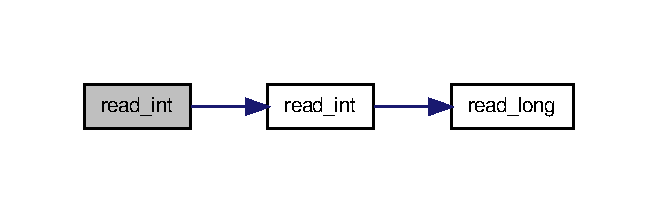
\includegraphics[width=350pt]{console__input_8h_a4f8c1bb51d432116d3eda43db3340c8c_cgraph}
\end{center}
\end{figure}


\hypertarget{console__input_8h_ad0ccfbb50d0e333ef8acfeab2b7d8071}{\index{console\-\_\-input.\-h@{console\-\_\-input.\-h}!read\-\_\-int@{read\-\_\-int}}
\index{read\-\_\-int@{read\-\_\-int}!console_input.h@{console\-\_\-input.\-h}}
\subsubsection[{read\-\_\-int}]{\setlength{\rightskip}{0pt plus 5cm}int read\-\_\-int (
\begin{DoxyParamCaption}
\item[{int}]{min, }
\item[{int}]{max}
\end{DoxyParamCaption}
)}}\label{console__input_8h_ad0ccfbb50d0e333ef8acfeab2b7d8071}
Reads a integer value in between a given interval from the console. When the entered value is not valid to the interval, the user gets prompted to reenter a valid.


\begin{DoxyParams}{Parameters}
{\em min} & lower bound of the interval. \\
\hline
{\em max} & top bound of the interval\\
\hline
\end{DoxyParams}
\begin{DoxyReturn}{Returns}
a int value in between min and max. 
\end{DoxyReturn}


Here is the call graph for this function\-:\nopagebreak
\begin{figure}[H]
\begin{center}
\leavevmode
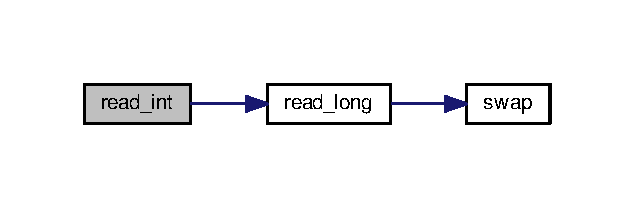
\includegraphics[width=334pt]{console__input_8h_ad0ccfbb50d0e333ef8acfeab2b7d8071_cgraph}
\end{center}
\end{figure}


\hypertarget{console__input_8h_aaaf3786f6b4803f3120609011de4b0db}{\index{console\-\_\-input.\-h@{console\-\_\-input.\-h}!read\-\_\-int@{read\-\_\-int}}
\index{read\-\_\-int@{read\-\_\-int}!console_input.h@{console\-\_\-input.\-h}}
\subsubsection[{read\-\_\-int}]{\setlength{\rightskip}{0pt plus 5cm}int read\-\_\-int (
\begin{DoxyParamCaption}
\item[{string}]{text}
\end{DoxyParamCaption}
)}}\label{console__input_8h_aaaf3786f6b4803f3120609011de4b0db}
Prints a text to the console and reads a integer value from the console in between the whole range of integer.


\begin{DoxyParams}{Parameters}
{\em text} & text to print to the console.\\
\hline
\end{DoxyParams}
\begin{DoxyReturn}{Returns}
a valid integer value. 
\end{DoxyReturn}


Here is the call graph for this function\-:\nopagebreak
\begin{figure}[H]
\begin{center}
\leavevmode
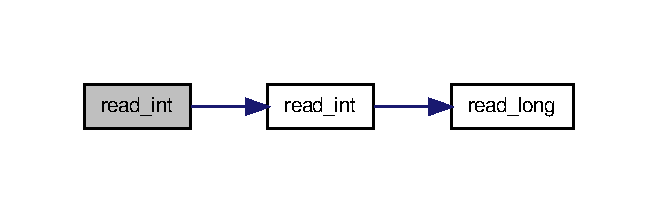
\includegraphics[width=350pt]{console__input_8h_aaaf3786f6b4803f3120609011de4b0db_cgraph}
\end{center}
\end{figure}


\hypertarget{console__input_8h_af310540093ee953c3018bc13bbde3da5}{\index{console\-\_\-input.\-h@{console\-\_\-input.\-h}!read\-\_\-int@{read\-\_\-int}}
\index{read\-\_\-int@{read\-\_\-int}!console_input.h@{console\-\_\-input.\-h}}
\subsubsection[{read\-\_\-int}]{\setlength{\rightskip}{0pt plus 5cm}int read\-\_\-int (
\begin{DoxyParamCaption}
{}
\end{DoxyParamCaption}
)}}\label{console__input_8h_af310540093ee953c3018bc13bbde3da5}
Reads an integer value from the terminal in between the whole range of long.

\begin{DoxyReturn}{Returns}
a valid integer value. 
\end{DoxyReturn}


Here is the call graph for this function\-:\nopagebreak
\begin{figure}[H]
\begin{center}
\leavevmode
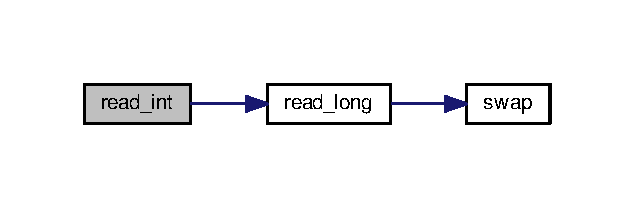
\includegraphics[width=334pt]{console__input_8h_af310540093ee953c3018bc13bbde3da5_cgraph}
\end{center}
\end{figure}


\hypertarget{console__input_8h_a03ebbd2a45117ee03be4e9002210ab36}{\index{console\-\_\-input.\-h@{console\-\_\-input.\-h}!read\-\_\-long@{read\-\_\-long}}
\index{read\-\_\-long@{read\-\_\-long}!console_input.h@{console\-\_\-input.\-h}}
\subsubsection[{read\-\_\-long}]{\setlength{\rightskip}{0pt plus 5cm}long read\-\_\-long (
\begin{DoxyParamCaption}
\item[{string}]{text, }
\item[{long}]{min, }
\item[{long}]{max}
\end{DoxyParamCaption}
)}}\label{console__input_8h_a03ebbd2a45117ee03be4e9002210ab36}
Prints a text to the console and reads a long value in between a given interval from the console. When the value is not in between the interval, the user gets prompted to reeinter a valid value.


\begin{DoxyParams}{Parameters}
{\em text} & text to print to the console. \\
\hline
{\em min} & lower bound of the interval. \\
\hline
{\em max} & top bound of the interval.\\
\hline
\end{DoxyParams}
\begin{DoxyReturn}{Returns}
a long value in between min and max. 
\end{DoxyReturn}


Here is the call graph for this function\-:\nopagebreak
\begin{figure}[H]
\begin{center}
\leavevmode
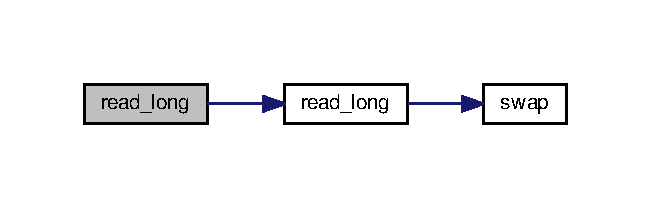
\includegraphics[width=342pt]{console__input_8h_a03ebbd2a45117ee03be4e9002210ab36_cgraph}
\end{center}
\end{figure}


\hypertarget{console__input_8h_a710a686867142de265860584f4147592}{\index{console\-\_\-input.\-h@{console\-\_\-input.\-h}!read\-\_\-long@{read\-\_\-long}}
\index{read\-\_\-long@{read\-\_\-long}!console_input.h@{console\-\_\-input.\-h}}
\subsubsection[{read\-\_\-long}]{\setlength{\rightskip}{0pt plus 5cm}long read\-\_\-long (
\begin{DoxyParamCaption}
\item[{long}]{min, }
\item[{long}]{max}
\end{DoxyParamCaption}
)}}\label{console__input_8h_a710a686867142de265860584f4147592}
Reads a long value in between a given interval from the console. When the entered value is not valid to the interval, the user gets prompted to reenter a valid.


\begin{DoxyParams}{Parameters}
{\em min} & lower bound of the interval. \\
\hline
{\em max} & top bound of the interval\\
\hline
\end{DoxyParams}
\begin{DoxyReturn}{Returns}
a long value in between min and max. 
\end{DoxyReturn}


Here is the call graph for this function\-:\nopagebreak
\begin{figure}[H]
\begin{center}
\leavevmode
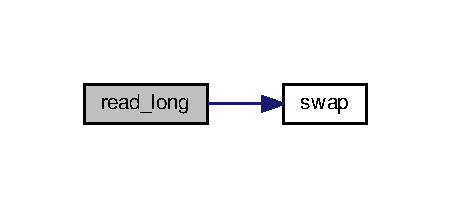
\includegraphics[width=246pt]{console__input_8h_a710a686867142de265860584f4147592_cgraph}
\end{center}
\end{figure}


\hypertarget{console__input_8h_a9128c63513d87af5259597d8c9930476}{\index{console\-\_\-input.\-h@{console\-\_\-input.\-h}!read\-\_\-long@{read\-\_\-long}}
\index{read\-\_\-long@{read\-\_\-long}!console_input.h@{console\-\_\-input.\-h}}
\subsubsection[{read\-\_\-long}]{\setlength{\rightskip}{0pt plus 5cm}long read\-\_\-long (
\begin{DoxyParamCaption}
\item[{string}]{text}
\end{DoxyParamCaption}
)}}\label{console__input_8h_a9128c63513d87af5259597d8c9930476}
Prints a text to the console and reads a long value from the console in between the whole range of long.


\begin{DoxyParams}{Parameters}
{\em text} & text to print to the console.\\
\hline
\end{DoxyParams}
\begin{DoxyReturn}{Returns}
a valid long value. 
\end{DoxyReturn}


Here is the call graph for this function\-:\nopagebreak
\begin{figure}[H]
\begin{center}
\leavevmode
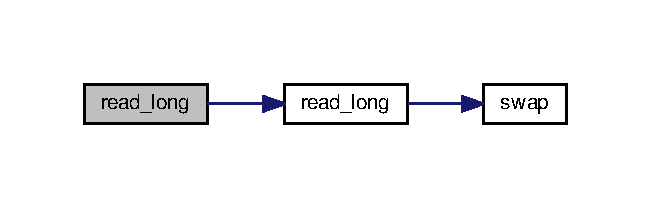
\includegraphics[width=342pt]{console__input_8h_a9128c63513d87af5259597d8c9930476_cgraph}
\end{center}
\end{figure}


\hypertarget{console__input_8h_a347c616893b725a74f60ea1f7ee325d2}{\index{console\-\_\-input.\-h@{console\-\_\-input.\-h}!read\-\_\-long@{read\-\_\-long}}
\index{read\-\_\-long@{read\-\_\-long}!console_input.h@{console\-\_\-input.\-h}}
\subsubsection[{read\-\_\-long}]{\setlength{\rightskip}{0pt plus 5cm}long read\-\_\-long (
\begin{DoxyParamCaption}
{}
\end{DoxyParamCaption}
)}}\label{console__input_8h_a347c616893b725a74f60ea1f7ee325d2}
Reads a long value from the terminal in between the whole range of long.

\begin{DoxyReturn}{Returns}
a valid long value. 
\end{DoxyReturn}


Here is the call graph for this function\-:\nopagebreak
\begin{figure}[H]
\begin{center}
\leavevmode
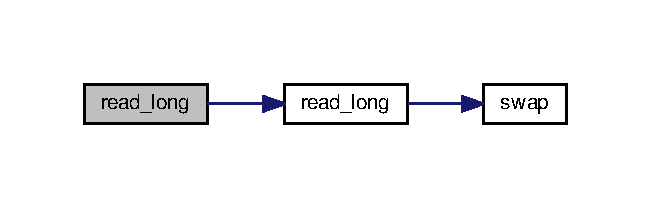
\includegraphics[width=342pt]{console__input_8h_a347c616893b725a74f60ea1f7ee325d2_cgraph}
\end{center}
\end{figure}


\hypertarget{console__input_8h_a44ccadd65be527f89bdcf6d27a3b1147}{\index{console\-\_\-input.\-h@{console\-\_\-input.\-h}!read\-\_\-text@{read\-\_\-text}}
\index{read\-\_\-text@{read\-\_\-text}!console_input.h@{console\-\_\-input.\-h}}
\subsubsection[{read\-\_\-text}]{\setlength{\rightskip}{0pt plus 5cm}string read\-\_\-text (
\begin{DoxyParamCaption}
\item[{string}]{text}
\end{DoxyParamCaption}
)}}\label{console__input_8h_a44ccadd65be527f89bdcf6d27a3b1147}
\hypertarget{console__input_8h_a6bac3909a28fff2736a171022343380b}{\index{console\-\_\-input.\-h@{console\-\_\-input.\-h}!read\-\_\-yes\-\_\-no@{read\-\_\-yes\-\_\-no}}
\index{read\-\_\-yes\-\_\-no@{read\-\_\-yes\-\_\-no}!console_input.h@{console\-\_\-input.\-h}}
\subsubsection[{read\-\_\-yes\-\_\-no}]{\setlength{\rightskip}{0pt plus 5cm}bool read\-\_\-yes\-\_\-no (
\begin{DoxyParamCaption}
\item[{string}]{text}
\end{DoxyParamCaption}
)}}\label{console__input_8h_a6bac3909a28fff2736a171022343380b}

\hypertarget{date_8h}{\section{date.\-h File Reference}
\label{date_8h}\index{date.\-h@{date.\-h}}
}
This graph shows which files directly or indirectly include this file\-:
\nopagebreak
\begin{figure}[H]
\begin{center}
\leavevmode
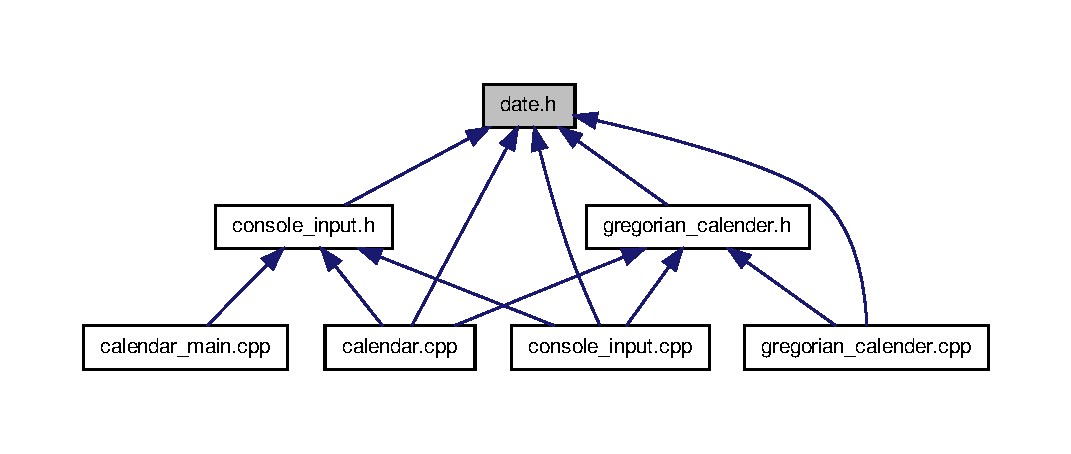
\includegraphics[width=350pt]{date_8h__dep__incl}
\end{center}
\end{figure}
\subsection*{Classes}
\begin{DoxyCompactItemize}
\item 
struct \hyperlink{structdate}{date}
\end{DoxyCompactItemize}
\subsection*{Typedefs}
\begin{DoxyCompactItemize}
\item 
typedef struct \hyperlink{structdate}{date} \hyperlink{date_8h_aeba59885914b6f3ad4be66c47fb8c8f2}{date}
\end{DoxyCompactItemize}


\subsection{Typedef Documentation}
\hypertarget{date_8h_aeba59885914b6f3ad4be66c47fb8c8f2}{\index{date.\-h@{date.\-h}!date@{date}}
\index{date@{date}!date.h@{date.\-h}}
\subsubsection[{date}]{\setlength{\rightskip}{0pt plus 5cm}typedef struct {\bf date}  {\bf date}}}\label{date_8h_aeba59885914b6f3ad4be66c47fb8c8f2}
Typedefinition of a struct Date. It consists of three integers\-: day, month and year. 
\hypertarget{gregorian__calender_8cpp}{\section{gregorian\-\_\-calender.\-cpp File Reference}
\label{gregorian__calender_8cpp}\index{gregorian\-\_\-calender.\-cpp@{gregorian\-\_\-calender.\-cpp}}
}
{\ttfamily \#include $<$iostream$>$}\\*
{\ttfamily \#include $<$iomanip$>$}\\*
{\ttfamily \#include \char`\"{}io\-\_\-util.\-h\char`\"{}}\\*
{\ttfamily \#include \char`\"{}date.\-h\char`\"{}}\\*
Include dependency graph for gregorian\-\_\-calender.\-cpp\-:
\nopagebreak
\begin{figure}[H]
\begin{center}
\leavevmode
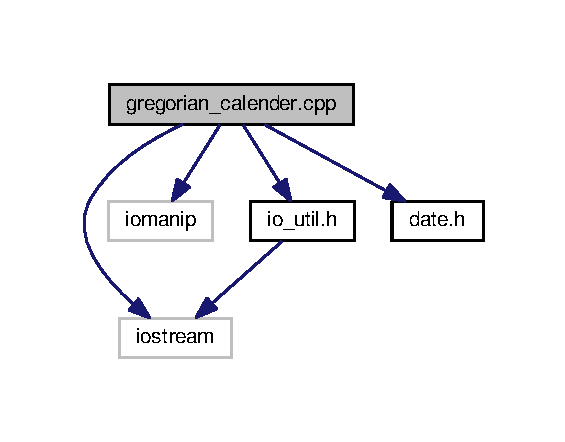
\includegraphics[width=271pt]{gregorian__calender_8cpp__incl}
\end{center}
\end{figure}
\subsection*{Functions}
\begin{DoxyCompactItemize}
\item 
bool \hyperlink{gregorian__calender_8cpp_ab345f7b66a3e361e0a77d7b7cbf235b9}{is\-\_\-leap\-\_\-year} (int year)
\item 
int \hyperlink{gregorian__calender_8cpp_ac931749f66720bdcba4d662b52d7de2b}{calc\-\_\-days\-\_\-of\-\_\-month} (int month, int year)
\item 
int \hyperlink{gregorian__calender_8cpp_a41d52c6b7790f79277145b6b1a67ee06}{calc\-\_\-days\-\_\-since\-\_\-the\-\_\-beginning} (int day, int month, int year)
\item 
int \hyperlink{gregorian__calender_8cpp_a14f3cbd497f4d93afc51445dc707b559}{calc\-\_\-days\-\_\-between\-\_\-dates} (\hyperlink{structDate}{Date} date1, \hyperlink{structDate}{Date} date2)
\item 
int \hyperlink{gregorian__calender_8cpp_a4c2416957da54061e0d8c03fff83d1a4}{calc\-\_\-start\-\_\-column} (int month, int year)
\item 
void \hyperlink{gregorian__calender_8cpp_aca17156e104486b3f78700b9c851f689}{print\-\_\-line} (char $\ast$sign, int length)
\item 
void \hyperlink{gregorian__calender_8cpp_a6b369b069a8ab93392690de255004d06}{print\-\_\-days} (int start\-\_\-column, int num\-\_\-days)
\item 
void \hyperlink{gregorian__calender_8cpp_af4184876e86f7f1935154dc22b034db0}{print\-\_\-calendar} (int month, int year)
\end{DoxyCompactItemize}


\subsection{Function Documentation}
\hypertarget{gregorian__calender_8cpp_a14f3cbd497f4d93afc51445dc707b559}{\index{gregorian\-\_\-calender.\-cpp@{gregorian\-\_\-calender.\-cpp}!calc\-\_\-days\-\_\-between\-\_\-dates@{calc\-\_\-days\-\_\-between\-\_\-dates}}
\index{calc\-\_\-days\-\_\-between\-\_\-dates@{calc\-\_\-days\-\_\-between\-\_\-dates}!gregorian_calender.cpp@{gregorian\-\_\-calender.\-cpp}}
\subsubsection[{calc\-\_\-days\-\_\-between\-\_\-dates}]{\setlength{\rightskip}{0pt plus 5cm}int calc\-\_\-days\-\_\-between\-\_\-dates (
\begin{DoxyParamCaption}
\item[{{\bf Date}}]{date1, }
\item[{{\bf Date}}]{date2}
\end{DoxyParamCaption}
)}}\label{gregorian__calender_8cpp_a14f3cbd497f4d93afc51445dc707b559}
Calculates the days in between two dates. The order of the dates is not important.


\begin{DoxyParams}{Parameters}
{\em date1} & first date to calculate days in between. \\
\hline
{\em date2} & second date to calculate days in between.\\
\hline
\end{DoxyParams}
\begin{DoxyReturn}{Returns}
days in between the given dates. 
\end{DoxyReturn}


Here is the call graph for this function\-:
\nopagebreak
\begin{figure}[H]
\begin{center}
\leavevmode
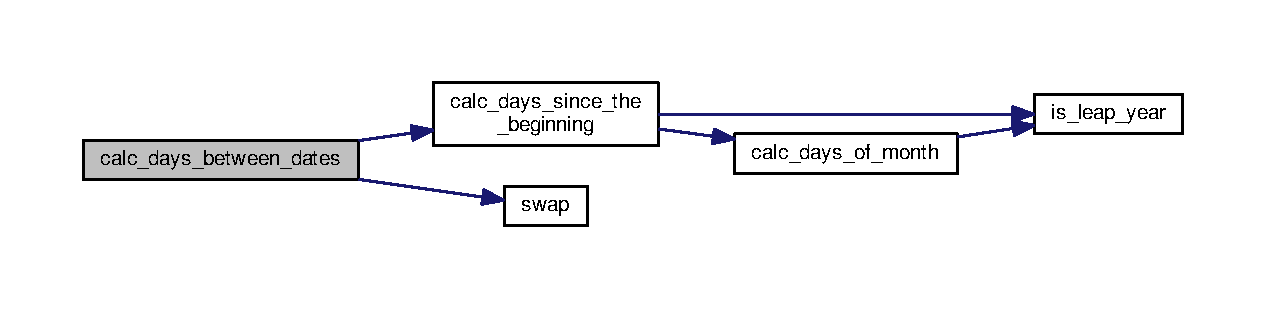
\includegraphics[width=350pt]{gregorian__calender_8cpp_a14f3cbd497f4d93afc51445dc707b559_cgraph}
\end{center}
\end{figure}


\hypertarget{gregorian__calender_8cpp_ac931749f66720bdcba4d662b52d7de2b}{\index{gregorian\-\_\-calender.\-cpp@{gregorian\-\_\-calender.\-cpp}!calc\-\_\-days\-\_\-of\-\_\-month@{calc\-\_\-days\-\_\-of\-\_\-month}}
\index{calc\-\_\-days\-\_\-of\-\_\-month@{calc\-\_\-days\-\_\-of\-\_\-month}!gregorian_calender.cpp@{gregorian\-\_\-calender.\-cpp}}
\subsubsection[{calc\-\_\-days\-\_\-of\-\_\-month}]{\setlength{\rightskip}{0pt plus 5cm}int calc\-\_\-days\-\_\-of\-\_\-month (
\begin{DoxyParamCaption}
\item[{int}]{month, }
\item[{int}]{year}
\end{DoxyParamCaption}
)}}\label{gregorian__calender_8cpp_ac931749f66720bdcba4d662b52d7de2b}
calcs the amount of days for the given month and year.


\begin{DoxyParams}{Parameters}
{\em month} & the month. \\
\hline
{\em year} & the year.\\
\hline
\end{DoxyParams}
\begin{DoxyReturn}{Returns}
amount the amount of days of the month. 
\end{DoxyReturn}


Here is the call graph for this function\-:
\nopagebreak
\begin{figure}[H]
\begin{center}
\leavevmode
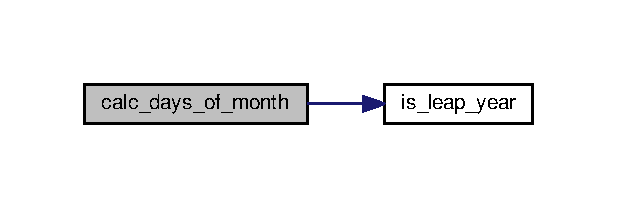
\includegraphics[width=296pt]{gregorian__calender_8cpp_ac931749f66720bdcba4d662b52d7de2b_cgraph}
\end{center}
\end{figure}


\hypertarget{gregorian__calender_8cpp_a41d52c6b7790f79277145b6b1a67ee06}{\index{gregorian\-\_\-calender.\-cpp@{gregorian\-\_\-calender.\-cpp}!calc\-\_\-days\-\_\-since\-\_\-the\-\_\-beginning@{calc\-\_\-days\-\_\-since\-\_\-the\-\_\-beginning}}
\index{calc\-\_\-days\-\_\-since\-\_\-the\-\_\-beginning@{calc\-\_\-days\-\_\-since\-\_\-the\-\_\-beginning}!gregorian_calender.cpp@{gregorian\-\_\-calender.\-cpp}}
\subsubsection[{calc\-\_\-days\-\_\-since\-\_\-the\-\_\-beginning}]{\setlength{\rightskip}{0pt plus 5cm}int calc\-\_\-days\-\_\-since\-\_\-the\-\_\-beginning (
\begin{DoxyParamCaption}
\item[{int}]{day, }
\item[{int}]{month, }
\item[{int}]{year}
\end{DoxyParamCaption}
)}}\label{gregorian__calender_8cpp_a41d52c6b7790f79277145b6b1a67ee06}
calc with a given date how many days are past since the 1.\-1.\-1583.


\begin{DoxyParams}{Parameters}
{\em day} & the day of the date. \\
\hline
{\em month} & the month of the date. \\
\hline
{\em year} & the year of the date.\\
\hline
\end{DoxyParams}
\begin{DoxyReturn}{Returns}
amount the amount days past since 1.\-1.\-1583. 
\end{DoxyReturn}


Here is the call graph for this function\-:
\nopagebreak
\begin{figure}[H]
\begin{center}
\leavevmode
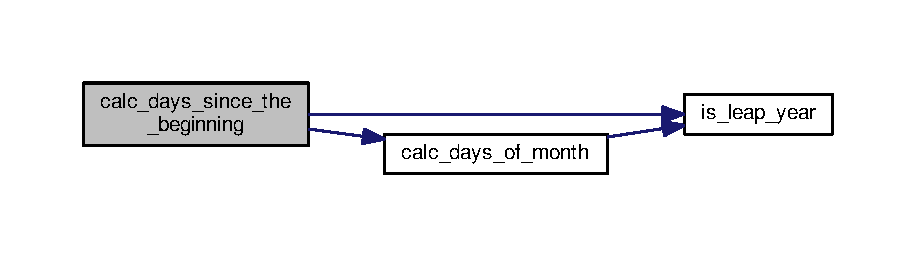
\includegraphics[width=350pt]{gregorian__calender_8cpp_a41d52c6b7790f79277145b6b1a67ee06_cgraph}
\end{center}
\end{figure}


\hypertarget{gregorian__calender_8cpp_a4c2416957da54061e0d8c03fff83d1a4}{\index{gregorian\-\_\-calender.\-cpp@{gregorian\-\_\-calender.\-cpp}!calc\-\_\-start\-\_\-column@{calc\-\_\-start\-\_\-column}}
\index{calc\-\_\-start\-\_\-column@{calc\-\_\-start\-\_\-column}!gregorian_calender.cpp@{gregorian\-\_\-calender.\-cpp}}
\subsubsection[{calc\-\_\-start\-\_\-column}]{\setlength{\rightskip}{0pt plus 5cm}int calc\-\_\-start\-\_\-column (
\begin{DoxyParamCaption}
\item[{int}]{month, }
\item[{int}]{year}
\end{DoxyParamCaption}
)}}\label{gregorian__calender_8cpp_a4c2416957da54061e0d8c03fff83d1a4}
Calculates for a given month and year the start column of a calendar for the first day of the month. The calendar starts with Sunday.

So $\vert$ Mo $\vert$ Di $\vert$ Mi $\vert$ Do $\vert$ Fr $\vert$ Sa 0 $\vert$ 1 $\vert$ 2 $\vert$ 3 $\vert$ 4 $\vert$ 5 $\vert$ 6


\begin{DoxyParams}{Parameters}
{\em month} & the given month. \\
\hline
{\em year} & the given year.\\
\hline
\end{DoxyParams}
\begin{DoxyReturn}{Returns}
the column in which the first year lies. 
\end{DoxyReturn}


Here is the call graph for this function\-:
\nopagebreak
\begin{figure}[H]
\begin{center}
\leavevmode
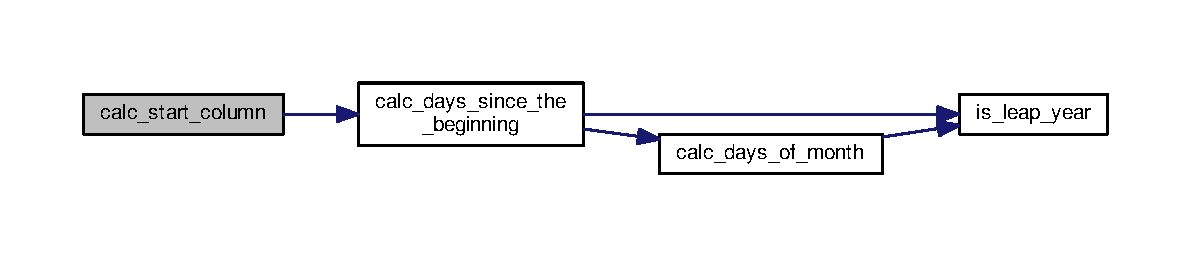
\includegraphics[width=350pt]{gregorian__calender_8cpp_a4c2416957da54061e0d8c03fff83d1a4_cgraph}
\end{center}
\end{figure}


\hypertarget{gregorian__calender_8cpp_ab345f7b66a3e361e0a77d7b7cbf235b9}{\index{gregorian\-\_\-calender.\-cpp@{gregorian\-\_\-calender.\-cpp}!is\-\_\-leap\-\_\-year@{is\-\_\-leap\-\_\-year}}
\index{is\-\_\-leap\-\_\-year@{is\-\_\-leap\-\_\-year}!gregorian_calender.cpp@{gregorian\-\_\-calender.\-cpp}}
\subsubsection[{is\-\_\-leap\-\_\-year}]{\setlength{\rightskip}{0pt plus 5cm}bool is\-\_\-leap\-\_\-year (
\begin{DoxyParamCaption}
\item[{int}]{year}
\end{DoxyParamCaption}
)}}\label{gregorian__calender_8cpp_ab345f7b66a3e361e0a77d7b7cbf235b9}
Checks if a year is a leap year.


\begin{DoxyParams}{Parameters}
{\em year} & the year to investigate.\\
\hline
\end{DoxyParams}
\begin{DoxyReturn}{Returns}
true if the year is a leap year. false if the year is not a leap year. 
\end{DoxyReturn}
\hypertarget{gregorian__calender_8cpp_af4184876e86f7f1935154dc22b034db0}{\index{gregorian\-\_\-calender.\-cpp@{gregorian\-\_\-calender.\-cpp}!print\-\_\-calendar@{print\-\_\-calendar}}
\index{print\-\_\-calendar@{print\-\_\-calendar}!gregorian_calender.cpp@{gregorian\-\_\-calender.\-cpp}}
\subsubsection[{print\-\_\-calendar}]{\setlength{\rightskip}{0pt plus 5cm}void print\-\_\-calendar (
\begin{DoxyParamCaption}
\item[{int}]{month, }
\item[{int}]{year}
\end{DoxyParamCaption}
)}}\label{gregorian__calender_8cpp_af4184876e86f7f1935154dc22b034db0}
Prints the calendar of a given month and year to the console.


\begin{DoxyParams}{Parameters}
{\em month} & month of the calendar. \\
\hline
{\em year} & year of the calendar. \\
\hline
\end{DoxyParams}


Here is the call graph for this function\-:
\nopagebreak
\begin{figure}[H]
\begin{center}
\leavevmode
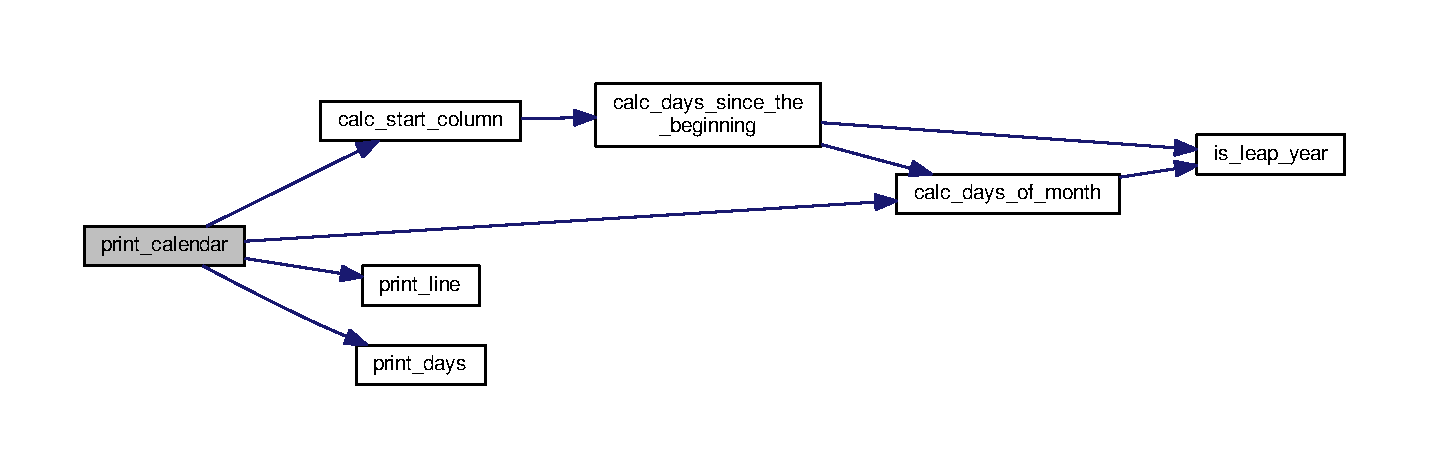
\includegraphics[width=350pt]{gregorian__calender_8cpp_af4184876e86f7f1935154dc22b034db0_cgraph}
\end{center}
\end{figure}


\hypertarget{gregorian__calender_8cpp_a6b369b069a8ab93392690de255004d06}{\index{gregorian\-\_\-calender.\-cpp@{gregorian\-\_\-calender.\-cpp}!print\-\_\-days@{print\-\_\-days}}
\index{print\-\_\-days@{print\-\_\-days}!gregorian_calender.cpp@{gregorian\-\_\-calender.\-cpp}}
\subsubsection[{print\-\_\-days}]{\setlength{\rightskip}{0pt plus 5cm}void print\-\_\-days (
\begin{DoxyParamCaption}
\item[{int}]{start\-\_\-column, }
\item[{int}]{num\-\_\-days}
\end{DoxyParamCaption}
)}}\label{gregorian__calender_8cpp_a6b369b069a8ab93392690de255004d06}
Prints days in the format of a Calendar to the console. Days before the start\-\_\-column are filled empty. \begin{DoxyVerb}  1     2    3     4     5     6
\end{DoxyVerb}
 7 8 9 10 11 12 13 14 15 16 17 18 19 20 21 22 23 24 25 26 27 28 29 30


\begin{DoxyParams}{Parameters}
{\em start\-\_\-column} & column of the first day. \\
\hline
{\em num\-\_\-days} & amount of days to print. \\
\hline
\end{DoxyParams}
\hypertarget{gregorian__calender_8cpp_aca17156e104486b3f78700b9c851f689}{\index{gregorian\-\_\-calender.\-cpp@{gregorian\-\_\-calender.\-cpp}!print\-\_\-line@{print\-\_\-line}}
\index{print\-\_\-line@{print\-\_\-line}!gregorian_calender.cpp@{gregorian\-\_\-calender.\-cpp}}
\subsubsection[{print\-\_\-line}]{\setlength{\rightskip}{0pt plus 5cm}void print\-\_\-line (
\begin{DoxyParamCaption}
\item[{char $\ast$}]{sign, }
\item[{int}]{length}
\end{DoxyParamCaption}
)}}\label{gregorian__calender_8cpp_aca17156e104486b3f78700b9c851f689}
Prints a line of a given sign for a given length to the console.


\begin{DoxyParams}{Parameters}
{\em sign} & sign to print the line with. \\
\hline
{\em length} & length of the line. \\
\hline
\end{DoxyParams}

\hypertarget{gregorian__calender_8h}{\section{gregorian\-\_\-calender.\-h File Reference}
\label{gregorian__calender_8h}\index{gregorian\-\_\-calender.\-h@{gregorian\-\_\-calender.\-h}}
}
{\ttfamily \#include \char`\"{}date.\-h\char`\"{}}\\*
Include dependency graph for gregorian\-\_\-calender.\-h\-:
\nopagebreak
\begin{figure}[H]
\begin{center}
\leavevmode
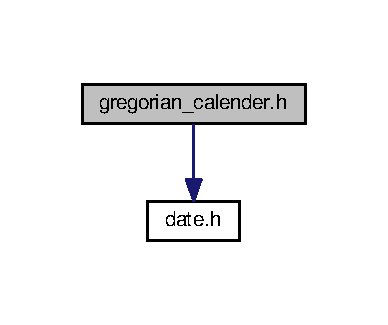
\includegraphics[width=186pt]{gregorian__calender_8h__incl}
\end{center}
\end{figure}
This graph shows which files directly or indirectly include this file\-:
\nopagebreak
\begin{figure}[H]
\begin{center}
\leavevmode
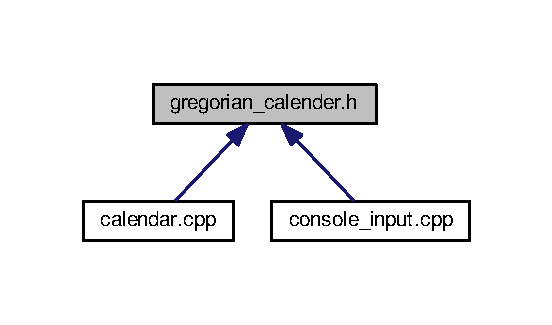
\includegraphics[width=265pt]{gregorian__calender_8h__dep__incl}
\end{center}
\end{figure}
\subsection*{Functions}
\begin{DoxyCompactItemize}
\item 
int \hyperlink{gregorian__calender_8h_ac931749f66720bdcba4d662b52d7de2b}{calc\-\_\-days\-\_\-of\-\_\-month} (int month, int year)
\item 
bool \hyperlink{gregorian__calender_8h_ab345f7b66a3e361e0a77d7b7cbf235b9}{is\-\_\-leap\-\_\-year} (int year)
\item 
int \hyperlink{gregorian__calender_8h_a41d52c6b7790f79277145b6b1a67ee06}{calc\-\_\-days\-\_\-since\-\_\-the\-\_\-beginning} (int day, int month, int year)
\item 
int \hyperlink{gregorian__calender_8h_a4c2416957da54061e0d8c03fff83d1a4}{calc\-\_\-start\-\_\-column} (int month, int year)
\item 
int \hyperlink{gregorian__calender_8h_a14f3cbd497f4d93afc51445dc707b559}{calc\-\_\-days\-\_\-between\-\_\-dates} (\hyperlink{structDate}{Date} date1, \hyperlink{structDate}{Date} date2)
\item 
void \hyperlink{gregorian__calender_8h_a10f558bb851e2d7fabc797845a157677}{print\-\_\-line} (int start\-\_\-column, int num\-\_\-days, int month, int year)
\item 
void \hyperlink{gregorian__calender_8h_a6b369b069a8ab93392690de255004d06}{print\-\_\-days} (int start\-\_\-column, int num\-\_\-days)
\item 
void \hyperlink{gregorian__calender_8h_aca17156e104486b3f78700b9c851f689}{print\-\_\-line} (char $\ast$sign, int length)
\item 
void \hyperlink{gregorian__calender_8h_af4184876e86f7f1935154dc22b034db0}{print\-\_\-calendar} (int month, int year)
\end{DoxyCompactItemize}


\subsection{Function Documentation}
\hypertarget{gregorian__calender_8h_a14f3cbd497f4d93afc51445dc707b559}{\index{gregorian\-\_\-calender.\-h@{gregorian\-\_\-calender.\-h}!calc\-\_\-days\-\_\-between\-\_\-dates@{calc\-\_\-days\-\_\-between\-\_\-dates}}
\index{calc\-\_\-days\-\_\-between\-\_\-dates@{calc\-\_\-days\-\_\-between\-\_\-dates}!gregorian_calender.h@{gregorian\-\_\-calender.\-h}}
\subsubsection[{calc\-\_\-days\-\_\-between\-\_\-dates}]{\setlength{\rightskip}{0pt plus 5cm}int calc\-\_\-days\-\_\-between\-\_\-dates (
\begin{DoxyParamCaption}
\item[{{\bf Date}}]{date1, }
\item[{{\bf Date}}]{date2}
\end{DoxyParamCaption}
)}}\label{gregorian__calender_8h_a14f3cbd497f4d93afc51445dc707b559}
Calculates the days in between two dates. The order of the dates is not important.


\begin{DoxyParams}{Parameters}
{\em date1} & first date to calculate days in between. \\
\hline
{\em date2} & second date to calculate days in between.\\
\hline
\end{DoxyParams}
\begin{DoxyReturn}{Returns}
days in between the given dates. 
\end{DoxyReturn}


Here is the call graph for this function\-:
\nopagebreak
\begin{figure}[H]
\begin{center}
\leavevmode
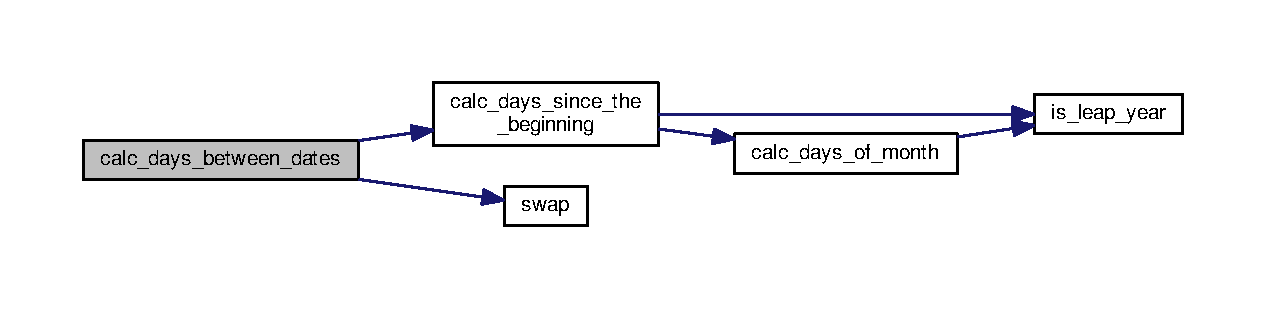
\includegraphics[width=350pt]{gregorian__calender_8h_a14f3cbd497f4d93afc51445dc707b559_cgraph}
\end{center}
\end{figure}


\hypertarget{gregorian__calender_8h_ac931749f66720bdcba4d662b52d7de2b}{\index{gregorian\-\_\-calender.\-h@{gregorian\-\_\-calender.\-h}!calc\-\_\-days\-\_\-of\-\_\-month@{calc\-\_\-days\-\_\-of\-\_\-month}}
\index{calc\-\_\-days\-\_\-of\-\_\-month@{calc\-\_\-days\-\_\-of\-\_\-month}!gregorian_calender.h@{gregorian\-\_\-calender.\-h}}
\subsubsection[{calc\-\_\-days\-\_\-of\-\_\-month}]{\setlength{\rightskip}{0pt plus 5cm}int calc\-\_\-days\-\_\-of\-\_\-month (
\begin{DoxyParamCaption}
\item[{int}]{month, }
\item[{int}]{year}
\end{DoxyParamCaption}
)}}\label{gregorian__calender_8h_ac931749f66720bdcba4d662b52d7de2b}
calcs the amount of days for the given month and year.


\begin{DoxyParams}{Parameters}
{\em month} & the month. \\
\hline
{\em year} & the year.\\
\hline
\end{DoxyParams}
\begin{DoxyReturn}{Returns}
amount the amount of days of the month. 
\end{DoxyReturn}


Here is the call graph for this function\-:
\nopagebreak
\begin{figure}[H]
\begin{center}
\leavevmode
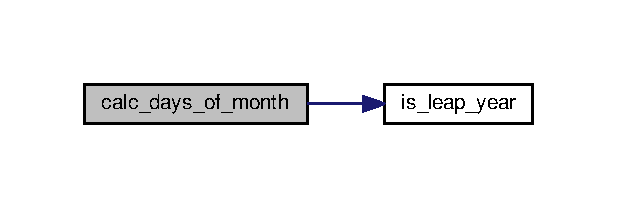
\includegraphics[width=296pt]{gregorian__calender_8h_ac931749f66720bdcba4d662b52d7de2b_cgraph}
\end{center}
\end{figure}


\hypertarget{gregorian__calender_8h_a41d52c6b7790f79277145b6b1a67ee06}{\index{gregorian\-\_\-calender.\-h@{gregorian\-\_\-calender.\-h}!calc\-\_\-days\-\_\-since\-\_\-the\-\_\-beginning@{calc\-\_\-days\-\_\-since\-\_\-the\-\_\-beginning}}
\index{calc\-\_\-days\-\_\-since\-\_\-the\-\_\-beginning@{calc\-\_\-days\-\_\-since\-\_\-the\-\_\-beginning}!gregorian_calender.h@{gregorian\-\_\-calender.\-h}}
\subsubsection[{calc\-\_\-days\-\_\-since\-\_\-the\-\_\-beginning}]{\setlength{\rightskip}{0pt plus 5cm}int calc\-\_\-days\-\_\-since\-\_\-the\-\_\-beginning (
\begin{DoxyParamCaption}
\item[{int}]{day, }
\item[{int}]{month, }
\item[{int}]{year}
\end{DoxyParamCaption}
)}}\label{gregorian__calender_8h_a41d52c6b7790f79277145b6b1a67ee06}
calc with a given date how many days are past since the 1.\-1.\-1583.


\begin{DoxyParams}{Parameters}
{\em day} & the day of the date. \\
\hline
{\em month} & the month of the date. \\
\hline
{\em year} & the year of the date.\\
\hline
\end{DoxyParams}
\begin{DoxyReturn}{Returns}
amount the amount days past since 1.\-1.\-1583. 
\end{DoxyReturn}


Here is the call graph for this function\-:
\nopagebreak
\begin{figure}[H]
\begin{center}
\leavevmode
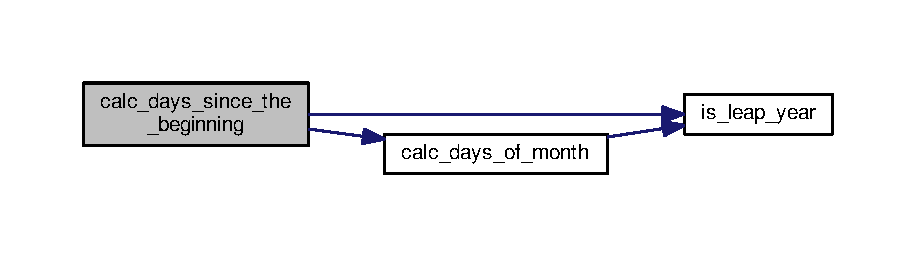
\includegraphics[width=350pt]{gregorian__calender_8h_a41d52c6b7790f79277145b6b1a67ee06_cgraph}
\end{center}
\end{figure}


\hypertarget{gregorian__calender_8h_a4c2416957da54061e0d8c03fff83d1a4}{\index{gregorian\-\_\-calender.\-h@{gregorian\-\_\-calender.\-h}!calc\-\_\-start\-\_\-column@{calc\-\_\-start\-\_\-column}}
\index{calc\-\_\-start\-\_\-column@{calc\-\_\-start\-\_\-column}!gregorian_calender.h@{gregorian\-\_\-calender.\-h}}
\subsubsection[{calc\-\_\-start\-\_\-column}]{\setlength{\rightskip}{0pt plus 5cm}int calc\-\_\-start\-\_\-column (
\begin{DoxyParamCaption}
\item[{int}]{month, }
\item[{int}]{year}
\end{DoxyParamCaption}
)}}\label{gregorian__calender_8h_a4c2416957da54061e0d8c03fff83d1a4}
Calculates for a given month and year the start column of a calendar for the first day of the month. The calendar starts with Sunday.

So $\vert$ Mo $\vert$ Di $\vert$ Mi $\vert$ Do $\vert$ Fr $\vert$ Sa 0 $\vert$ 1 $\vert$ 2 $\vert$ 3 $\vert$ 4 $\vert$ 5 $\vert$ 6


\begin{DoxyParams}{Parameters}
{\em month} & the given month. \\
\hline
{\em year} & the given year.\\
\hline
\end{DoxyParams}
\begin{DoxyReturn}{Returns}
the column in which the first year lies. 
\end{DoxyReturn}


Here is the call graph for this function\-:
\nopagebreak
\begin{figure}[H]
\begin{center}
\leavevmode
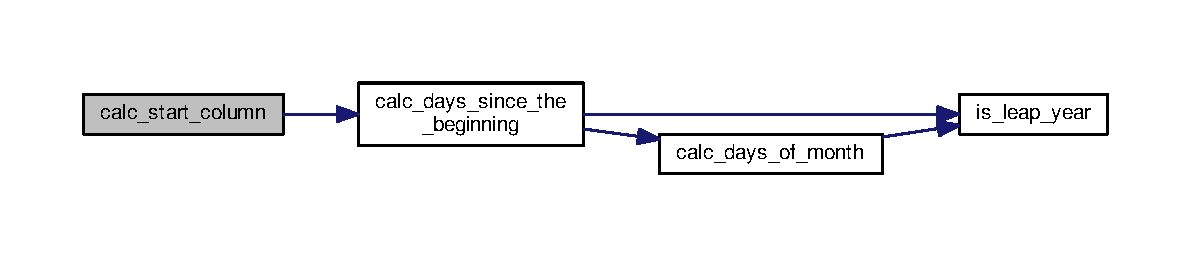
\includegraphics[width=350pt]{gregorian__calender_8h_a4c2416957da54061e0d8c03fff83d1a4_cgraph}
\end{center}
\end{figure}


\hypertarget{gregorian__calender_8h_ab345f7b66a3e361e0a77d7b7cbf235b9}{\index{gregorian\-\_\-calender.\-h@{gregorian\-\_\-calender.\-h}!is\-\_\-leap\-\_\-year@{is\-\_\-leap\-\_\-year}}
\index{is\-\_\-leap\-\_\-year@{is\-\_\-leap\-\_\-year}!gregorian_calender.h@{gregorian\-\_\-calender.\-h}}
\subsubsection[{is\-\_\-leap\-\_\-year}]{\setlength{\rightskip}{0pt plus 5cm}bool is\-\_\-leap\-\_\-year (
\begin{DoxyParamCaption}
\item[{int}]{year}
\end{DoxyParamCaption}
)}}\label{gregorian__calender_8h_ab345f7b66a3e361e0a77d7b7cbf235b9}
Checks if a year is a leap year.


\begin{DoxyParams}{Parameters}
{\em year} & the year to investigate.\\
\hline
\end{DoxyParams}
\begin{DoxyReturn}{Returns}
true if the year is a leap year. false if the year is not a leap year. 
\end{DoxyReturn}
\hypertarget{gregorian__calender_8h_af4184876e86f7f1935154dc22b034db0}{\index{gregorian\-\_\-calender.\-h@{gregorian\-\_\-calender.\-h}!print\-\_\-calendar@{print\-\_\-calendar}}
\index{print\-\_\-calendar@{print\-\_\-calendar}!gregorian_calender.h@{gregorian\-\_\-calender.\-h}}
\subsubsection[{print\-\_\-calendar}]{\setlength{\rightskip}{0pt plus 5cm}void print\-\_\-calendar (
\begin{DoxyParamCaption}
\item[{int}]{month, }
\item[{int}]{year}
\end{DoxyParamCaption}
)}}\label{gregorian__calender_8h_af4184876e86f7f1935154dc22b034db0}
Prints the calendar of a given month and year to the console.


\begin{DoxyParams}{Parameters}
{\em month} & month of the calendar. \\
\hline
{\em year} & year of the calendar. \\
\hline
\end{DoxyParams}


Here is the call graph for this function\-:
\nopagebreak
\begin{figure}[H]
\begin{center}
\leavevmode
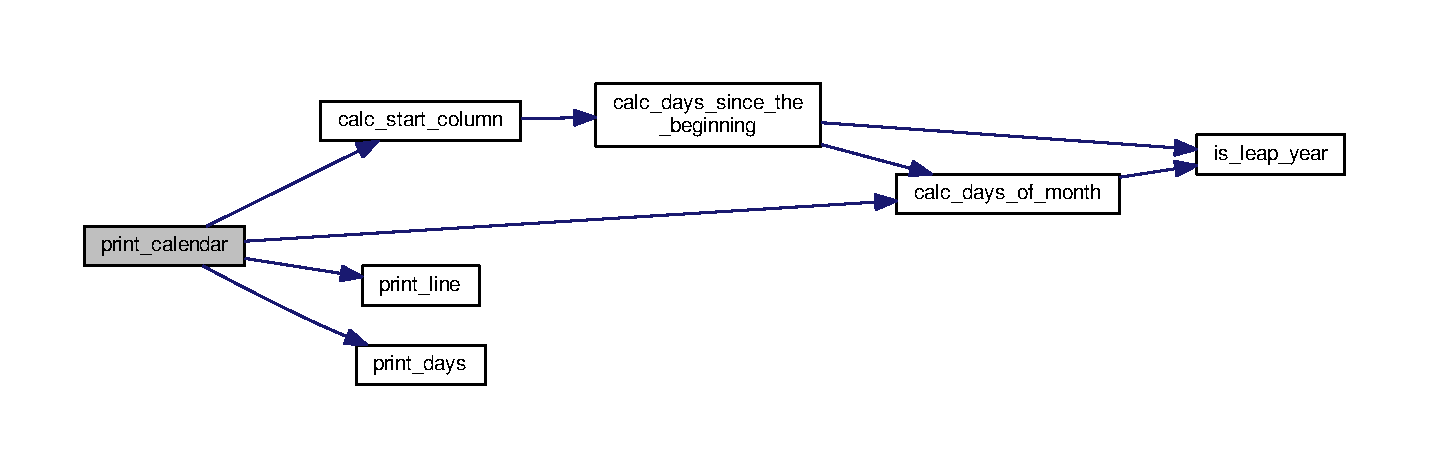
\includegraphics[width=350pt]{gregorian__calender_8h_af4184876e86f7f1935154dc22b034db0_cgraph}
\end{center}
\end{figure}


\hypertarget{gregorian__calender_8h_a6b369b069a8ab93392690de255004d06}{\index{gregorian\-\_\-calender.\-h@{gregorian\-\_\-calender.\-h}!print\-\_\-days@{print\-\_\-days}}
\index{print\-\_\-days@{print\-\_\-days}!gregorian_calender.h@{gregorian\-\_\-calender.\-h}}
\subsubsection[{print\-\_\-days}]{\setlength{\rightskip}{0pt plus 5cm}void print\-\_\-days (
\begin{DoxyParamCaption}
\item[{int}]{start\-\_\-column, }
\item[{int}]{num\-\_\-days}
\end{DoxyParamCaption}
)}}\label{gregorian__calender_8h_a6b369b069a8ab93392690de255004d06}
Prints days in the format of a Calendar to the console. Days before the start\-\_\-column are filled empty. \begin{DoxyVerb}  1     2    3     4     5     6
\end{DoxyVerb}
 7 8 9 10 11 12 13 14 15 16 17 18 19 20 21 22 23 24 25 26 27 28 29 30


\begin{DoxyParams}{Parameters}
{\em start\-\_\-column} & column of the first day. \\
\hline
{\em num\-\_\-days} & amount of days to print. \\
\hline
\end{DoxyParams}
\hypertarget{gregorian__calender_8h_a10f558bb851e2d7fabc797845a157677}{\index{gregorian\-\_\-calender.\-h@{gregorian\-\_\-calender.\-h}!print\-\_\-line@{print\-\_\-line}}
\index{print\-\_\-line@{print\-\_\-line}!gregorian_calender.h@{gregorian\-\_\-calender.\-h}}
\subsubsection[{print\-\_\-line}]{\setlength{\rightskip}{0pt plus 5cm}void print\-\_\-line (
\begin{DoxyParamCaption}
\item[{int}]{start\-\_\-column, }
\item[{int}]{num\-\_\-days, }
\item[{int}]{month, }
\item[{int}]{year}
\end{DoxyParamCaption}
)}}\label{gregorian__calender_8h_a10f558bb851e2d7fabc797845a157677}
\hypertarget{gregorian__calender_8h_aca17156e104486b3f78700b9c851f689}{\index{gregorian\-\_\-calender.\-h@{gregorian\-\_\-calender.\-h}!print\-\_\-line@{print\-\_\-line}}
\index{print\-\_\-line@{print\-\_\-line}!gregorian_calender.h@{gregorian\-\_\-calender.\-h}}
\subsubsection[{print\-\_\-line}]{\setlength{\rightskip}{0pt plus 5cm}void print\-\_\-line (
\begin{DoxyParamCaption}
\item[{char $\ast$}]{sign, }
\item[{int}]{length}
\end{DoxyParamCaption}
)}}\label{gregorian__calender_8h_aca17156e104486b3f78700b9c851f689}
Prints a line of a given sign for a given length to the console.


\begin{DoxyParams}{Parameters}
{\em sign} & sign to print the line with. \\
\hline
{\em length} & length of the line. \\
\hline
\end{DoxyParams}

\hypertarget{io__util_8cpp}{\section{io\-\_\-util.\-cpp File Reference}
\label{io__util_8cpp}\index{io\-\_\-util.\-cpp@{io\-\_\-util.\-cpp}}
}
{\ttfamily \#include $<$iostream$>$}\\*
Include dependency graph for io\-\_\-util.\-cpp\-:
\nopagebreak
\begin{figure}[H]
\begin{center}
\leavevmode
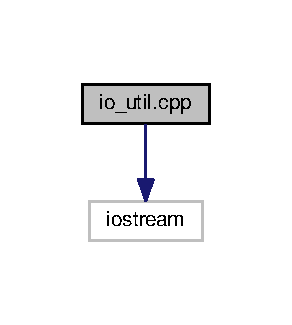
\includegraphics[width=140pt]{io__util_8cpp__incl}
\end{center}
\end{figure}
\subsection*{Functions}
\begin{DoxyCompactItemize}
\item 
void \hyperlink{io__util_8cpp_ae8c346aa92fc891022a940f2c5c75f95}{setze\-\_\-schalter} (ios\-\_\-base\-::fmtflags format)
\item 
void \hyperlink{io__util_8cpp_acd3415eef442ced2b5e064f95f04b624}{swap} (int $\ast$x, int $\ast$y)
\end{DoxyCompactItemize}


\subsection{Function Documentation}
\hypertarget{io__util_8cpp_ae8c346aa92fc891022a940f2c5c75f95}{\index{io\-\_\-util.\-cpp@{io\-\_\-util.\-cpp}!setze\-\_\-schalter@{setze\-\_\-schalter}}
\index{setze\-\_\-schalter@{setze\-\_\-schalter}!io_util.cpp@{io\-\_\-util.\-cpp}}
\subsubsection[{setze\-\_\-schalter}]{\setlength{\rightskip}{0pt plus 5cm}void setze\-\_\-schalter (
\begin{DoxyParamCaption}
\item[{ios\-\_\-base\-::fmtflags}]{format}
\end{DoxyParamCaption}
)}}\label{io__util_8cpp_ae8c346aa92fc891022a940f2c5c75f95}
\hypertarget{io__util_8cpp_acd3415eef442ced2b5e064f95f04b624}{\index{io\-\_\-util.\-cpp@{io\-\_\-util.\-cpp}!swap@{swap}}
\index{swap@{swap}!io_util.cpp@{io\-\_\-util.\-cpp}}
\subsubsection[{swap}]{\setlength{\rightskip}{0pt plus 5cm}void swap (
\begin{DoxyParamCaption}
\item[{int $\ast$}]{x, }
\item[{int $\ast$}]{y}
\end{DoxyParamCaption}
)}}\label{io__util_8cpp_acd3415eef442ced2b5e064f95f04b624}

\hypertarget{io__util_8h}{\section{io\-\_\-util.\-h File Reference}
\label{io__util_8h}\index{io\-\_\-util.\-h@{io\-\_\-util.\-h}}
}
{\ttfamily \#include $<$iostream$>$}\\*
Include dependency graph for io\-\_\-util.\-h\-:
\nopagebreak
\begin{figure}[H]
\begin{center}
\leavevmode
\includegraphics[width=134pt]{io__util_8h__incl}
\end{center}
\end{figure}
This graph shows which files directly or indirectly include this file\-:
\nopagebreak
\begin{figure}[H]
\begin{center}
\leavevmode
\includegraphics[width=309pt]{io__util_8h__dep__incl}
\end{center}
\end{figure}
\subsection*{Functions}
\begin{DoxyCompactItemize}
\item 
void \hyperlink{io__util_8h_ae8c346aa92fc891022a940f2c5c75f95}{setze\-\_\-schalter} (ios\-\_\-base\-::fmtflags format)
\item 
void \hyperlink{io__util_8h_acd3415eef442ced2b5e064f95f04b624}{swap} (int $\ast$x, int $\ast$y)
\end{DoxyCompactItemize}


\subsection{Function Documentation}
\hypertarget{io__util_8h_ae8c346aa92fc891022a940f2c5c75f95}{\index{io\-\_\-util.\-h@{io\-\_\-util.\-h}!setze\-\_\-schalter@{setze\-\_\-schalter}}
\index{setze\-\_\-schalter@{setze\-\_\-schalter}!io_util.h@{io\-\_\-util.\-h}}
\subsubsection[{setze\-\_\-schalter}]{\setlength{\rightskip}{0pt plus 5cm}void setze\-\_\-schalter (
\begin{DoxyParamCaption}
\item[{ios\-\_\-base\-::fmtflags}]{format}
\end{DoxyParamCaption}
)}}\label{io__util_8h_ae8c346aa92fc891022a940f2c5c75f95}
\hypertarget{io__util_8h_acd3415eef442ced2b5e064f95f04b624}{\index{io\-\_\-util.\-h@{io\-\_\-util.\-h}!swap@{swap}}
\index{swap@{swap}!io_util.h@{io\-\_\-util.\-h}}
\subsubsection[{swap}]{\setlength{\rightskip}{0pt plus 5cm}void swap (
\begin{DoxyParamCaption}
\item[{int $\ast$}]{x, }
\item[{int $\ast$}]{y}
\end{DoxyParamCaption}
)}}\label{io__util_8h_acd3415eef442ced2b5e064f95f04b624}

%--- End generated contents ---

% Index
\newpage
\phantomsection
\addcontentsline{toc}{chapter}{Index}
\printindex

\end{document}
